% ULaTeX2e, calling the article.cls class and 12-point type.

\documentclass[12pt]{article}

% My packages

\usepackage{amsmath}
\usepackage{framed, color}
\usepackage{soul}
\definecolor{blu}{rgb}{0,0,1}
\newcommand{\td}[1]{{\color{blu}\hl{TODO: #1}}}
\usepackage{graphicx}
\usepackage{amsthm}
\newtheorem{mydef}{Definition}
\usepackage{dcolumn}
\usepackage{multirow}
\usepackage{booktabs}
\newcolumntype{d}{D{.}{.}{4.0}}
\newcolumntype{s}{D{.}{.}{1.4}}

\usepackage{arydshln}

% Users of the {thebibliography} environment or BibTeX should use the
% scicite.sty package, downloadable from *Science* at
% www.sciencemag.org/about/authors/prep/TeX_help/ .
% This package should properly format in-text
% reference calls and reference-list numbers.

\usepackage{scicite}

% Use times if you have the font installed; otherwise, comment out the
% following line.

\usepackage{times}

% The preamble here sets up a lot of new/revised commands and
% environments.  It's annoying, but please do *not* try to strip these
% out into a separate .sty file (which could lead to the loss of some
% information when we convert the file to other formats).  Instead, keep
% them in the preamble of your main LaTeX source file.


% The following parameters seem to provide a reasonable page setup.

\topmargin 0.0cm
\oddsidemargin 0.2cm
\textwidth 16cm 
\textheight 21cm
\footskip 1.0cm


%The next command sets up an environment for the abstract to your paper.

\newenvironment{sciabstract}{%
\begin{quote} \bf}
{\end{quote}}


% If your reference list includes text notes as well as references,
% include the following line; otherwise, comment it out.

\renewcommand\refname{References and Notes}

% The following lines set up an environment for the last note in the
% reference list, which commonly includes acknowledgments of funding,
% help, etc.  It's intended for users of BibTeX or the {thebibliography}
% environment.  Users who are hand-coding their references at the end
% using a list environment such as {enumerate} can simply add another
% item at the end, and it will be numbered automatically.

\newcounter{lastnote}
\newenvironment{scilastnote}{%
\setcounter{lastnote}{\value{enumiv}}%
\addtocounter{lastnote}{+1}%
\begin{list}%
{\arabic{lastnote}.}
{\setlength{\leftmargin}{.22in}}
{\setlength{\labelsep}{.5em}}}
{\end{list}}


% Include your paper's title here

\title{Hysteresis in human computation:\\ how one task affects another} 


% Place the author information here.  Please hand-code the contact
% information and notecalls; do *not* use \footnote commands.  Let the
% author contact information appear immediately below the author names
% as shown.  We would also prefer that you don't change the type-size
% settings shown here.

\author
{Edward Newell \\ Derek Ruths\\
\\
\normalsize{\texttt{edward.newell@mail.mcgill.ca}}\\
\normalsize{\texttt{derek.ruths@mcgill.ca}}\\
\normalsize{School of Computer Science, McGill University,}\\
\normalsize{3480 University Street, Room 318, Montreal, Quebec, Canada, H3A 2A7}\\
\\
}




% Include the date command, but leave its argument blank.

\date{}



%%%%%%%%%%%%%%%%% END OF PREAMBLE %%%%%%%%%%%%%%%%



\begin{document} 

% Double-space the manuscript.

\baselineskip24pt

% Make the title.

\maketitle 



% Place your abstract within the special {sciabstract} environment.

\begin{sciabstract}
Microtask platforms have become commonplace tools for obtaining human 
annotations for large datasets.  Such platforms connect requesters 
(researchers or companies) with large populations (crowds) of workers, who 
will individually complete small information-processing jobs, each taking 
typically between one to five minutes.  
A major challenge in using such platforms, 
and a topic of ongoing research, concerns designing jobs that elicit high 
quality annotations. Here we identify a feature of nearly all crowdsourcing 
jobs that can act as a strong and systemic source of bias in annotations 
produced by workers. Specifically, many microtask jobs consist of a sequence 
of tasks which share a common format (e.g., label pictures, identify people, 
circle galaxies). Using image-labeling, a canonical microtask job format, we 
discover that earlier tasks shift the distribution of future answers by 
30-50\%. 
Moreover, we show that prior tasks influence 
the content that workers chose to focus on, as well as the richness and 
specialization of their word choice. While these intertask effects can be a 
source of systematic bias, our results suggest that, with appropriate job 
design, it might be possible to leverage these biases to hone worker focus 
and specificity, helping to elicit reproducible, expert-level judgments.
\end{sciabstract}

\section*{Main text}
Microtask platforms are online marketplaces in which \textit{requesters} 
post batches of tasks, and \textit{workers} complete them
for remuneration, a sense of purpose, and fun
\cite{kazai2013analysis,Antin20122925}.
Typical tasks include tagging and categorizing images 
\cite{6116320,Zhai2012357}, coding and transcription, such as of voice recordings or handwritten notes
\cite{chandler2013breaking,paolacci2010running,Berinsky2012351,Finnerty2013}, 
and judging relevancy and quality, for example, to rate information 
retrieval systems \cite{le2010ensuring,grady2010crowdsourcing,alonso2009can,kazai2013analysis}.

In this form of crowdsourcing, workers appear like input-output devices.  
Such platforms provide much of the flexibility and 
cost-savings of fully automating the work in a computer program: 
the workforce is available on demand over the Internet using automated 
scripts, and  no interviews or contracts are required 
\cite{wolfson2011look,5543192}.  Many tasks
can be performed at a fraction of the cost of traditional methods for 
recruiting temporary workers or experimental subjects
\cite{Berinsky2012351,paolacci2010running,ranade2012crowdsource}.
From the requester's perspective, using microtask platforms resembles
running a computer program on a remote server, leading some to investigate
these platforms as a new computing architecture \cite{5543192,little2010turkit,minder2012crowdlang,kittur2011crowdforge}.

Due to its flexibility and cost-effectiveness, 
there has been a surge in demand for microtask work
in both industry and academia\cite{wolfson2011look,Berinsky2012351}.  
Naturally, there is a desire to understand the factors affecting the 
reliability of microtask-based methods.  Researchers have investigated 
task-design parameters such as the 
level of pay \cite{Mason200977,kazai2013analysis}, 
the training and pre-screening of workers 
\cite{le2010ensuring,paolacci2010running,kazai2013analysis}, 
user-interface design \cite{Finnerty2013}, and timely feedback 
\cite{Dow20121013}.
Researchers have also investigated the effects of \textit{framing}, 
by altering the description of the workflow context 
\cite{Kinnaird2012281}, the purpose of tasks 
\cite{chandler2013breaking}, and the problem description
\cite{thibodeau2013natural}.  Another important avenue of research concerns
workflow design: how to break down a complex problem into microtasks
\cite{kittur2011crowdforge}, the effect of microtask size 
\cite{Huang201077}, and the effects of interruptions \cite{laseckieffects}.

Here, we focus on a ubiquitous feature of microtask work: the tendency
for workers to perform many similar tasks in quick succession.  
To describe this tendency, it is necessary to clarify terminology.
On one popular microtask platform, Amazon's Mechanical Turk (MTurk), 
tasks are delivered in bundles called Human Intelligence Tasks (HITs).  
But for clarity, we will use ``task'' to mean 
the smallest repeatable unit of work; for example, labeling one image with
some descriptive words (\textit{labels}).  
Using this terminology, it is typical for a HIT to
actually consist of \textit{several tasks}, 
such as labeling ten images consecutively.

In addition to the task-repetition occuring \textit{within} HITs, 
workers prefer HITs that are part of a large set of HITs
having the same format, and cite speed and repeatability 
as desireable traits \cite{Chilton20101}.  When the tasks in a sequence are 
sufficiently similar, workers are more efficient \cite{laseckieffects}, 
and the cognitive load resulting from task-switching \cite{Adamczyk2004271} 
is eliminated.  Meanwhile, breaking complex jobs down into simpler tasks 
appears to improve results \cite{kittur2011crowdforge}.  
Thus, from the perspectives of both the worker and requester, 
it is desireable for workers to perform repetitive sequences of similar 
tasks in quick succession.

The repetitive completion of tasks is of concern because people's responses
to a prompt can be strongly influenced by their recent exposure to stimuli,
due to the well-known phenomenon of \textit{priming} 
\cite{BJOP1796,No2007,beller1971priming}.  Priming is typically relevant when 
the prior stimuli bear some conceptual or perceptual connection to the 
ensuing task\cite{Gass1999549,sohn2001task}, and so, the repetition of 
similar tasks within the typical microtask setup creates an ideal context for 
strong priming effects.

Researchers investigating a somewhat similar class of psychological phenomena,
found that ratings that microtask workers give to items in a list
depend on the order in which the list is presented, an effect known as
\textit{positional bias} \cite{lerman2014leveraging}.  This serves as an 
example of a basic psychological phenomenon impacting crowdsourced data,
and raises questions about what other cognitive biases might
affect microtask work, and how prevalent the induced bias might be.  

Here we investigate the potential for task-repetition to induce bias in 
microtask-based work in a highly generalizeable setting.  
If such bias is present, it would impact virtually 
every microtask and crowdsourced workflow.
Our results show that a worker's response during a task
does indeed depend strongly on the tasks performed beforehand.   
We call the effects that earlier tasks exert on later ones 
\textit{intertask effects}.

As we have described, microtask platforms have been widely adopted as a 
tool, but computer scientists also hold such platforms as the object of 
research, viewing  microtask platforms as a new kind of computing 
architecture.  In analogy to CPUs (central 
processing units) and GPUs (graphics processing units), 
Davis \textit{et al} invoked the \textit{human processing unit}, or HPU \cite{5543192}.
Researchers have sought to define a set of basic HPU operations, and
have developed libraries and frameworks to simplify HPU programming 
and make it more like CPU programming 
\cite{little2010turkit,minder2012crowdlang,kittur2011crowdforge}.  
As an example, one operation overcomes the inherent stochasticity of HPU 
outputs, by automatically aggregating votes from multiple HPUs under a single
function call.  

But our revelation of strong intertask effects shows that, 
in addition to stochasticity, HPUs are subject to \textit{hysteresis}, 
meaning that their 
outputs depend on the history of their inputs.  Reproducibility and 
path-independence are crucial properties for the components of a 
computing architecture, so a better understanding of the computational 
ramifications of many psychological phenomena is needed. 

We investigated intertask effects using image-labeling tasks on the Amazon 
Mechanical Turk (MTurk) microtask platform.  
In addition to being one of the most common kinds of tasks
\cite{chandler2013breaking,Berinsky2012351,Finnerty2013,paolacci2010running},
image-labeling is prototypical for any kind of task in which the worker is 
asked to provide a high-level judgment, incorporating prior knowledge, in 
response to a prompt.  
This includes such diverse tasks as describing
video and audio recordings, summarizing texts, or providing feedback to a 
product review.

In our first experiment, which we call
\textit{intertask-food-objects}, workers were assigned to either a
\textit{food} or \textit{objects} treatment.  Workers in these treatments
performed a set of five \textit{initial tasks}, which each involved 
providing five descriptive labels for an image depicting 
either food or (non-food) objects, depending on the worker's 
treatment (Fig.~\ref{fig:task}A and B).  Following the initial 
tasks, workers performed five \textit{test tasks}, which were identical for 
both treatments.  The test tasks contained images depicting a 
mixture of food and objects (Fig.~\ref{fig:task}C), and workers
were again asked to provide five labels for each.  Five initial 
tasks, together with the test tasks, comprised one HIT\footnote{
	Workers were only allowed to participate in one HIT relating to this study.
}. During the HIT, workers 
were presented images one at a time, and, crucially, we made no 
distinction between the initial and test tasks.

A $\chi^2$ test shows that the frequencies of words used by
workers in the \textit{food} and \textit{objects} treatments differed
significantly during test tasks ($p = 6.0 \times 10^{-14}$), even though the test tasks were identical 
in both treatments\footnote{see supplementary text for tabulated statistics.}.  This shows that earlier tasks have a 
significant effect on later ones, and raises concerns about the 
design of microtasks, and possibly the microtask methodology itself.

While this affirms the \textit{existence} of intertask effects, we wish to
understand the nature and severity of the bias induced by prior task 
exposures.  To this end, we define the extent of bias, $\theta$, in terms of
the strength of influence that a perturbation has on worker's responses.
Since workers' responses are stochastic, we define the extent of bias in 
terms of the shift induced in the distribution of responses\footnote{
	This is a general divergence metric between probability 
	distributions known as the \textit{total variation distance.}
}:
\begin{equation}
	\theta = \frac{1}{2}\sum_{x \in X} \left| p_0(x) - p_1(x) \right|,
	\label{eq:theta}
\end{equation}
where $p_i(x)$ is the probability that a worker subjected to treatment $i$
provides response $x$, from the set of possible responses $X$.
It is important to emphasize that a significant result from a $\chi^2$ test 
only allows us to conclude that $\theta$ is non-zero 
(see supplementary text).  
Determining $\theta$ from finite samples of responses, using purely 
statistical approaches, is difficult (see supplementary text),
which leads us to reformulate the
problem in terms of classification: given a worker's 
responses to test tasks, can a machine reliably infer what her prior exposure 
had been?  Intuitively, the greater the effect that prior tasks have on 
subsequent
responses, the more accurate the classifier can be.  Formally (as shown
in the supplementary text), the accuracy of such a classifier, $\eta$,
yields a lower bound on the bias:
\begin{equation}
	\theta \geq 2\eta - 1.
	\label{l1}
\end{equation}
By measuring the accuracy of a classifier, we can bound the 
bias induced by any perturbation, including both intertask effects and 
framing.  As defined, bias ranges from 0 (meaning the exposures 
does not affect the distribution of responses), to 1 
(or 100\%) (meaning that the exposure leads workers to provide a completely
different set of responses).

\begin{figure}
	\centering
	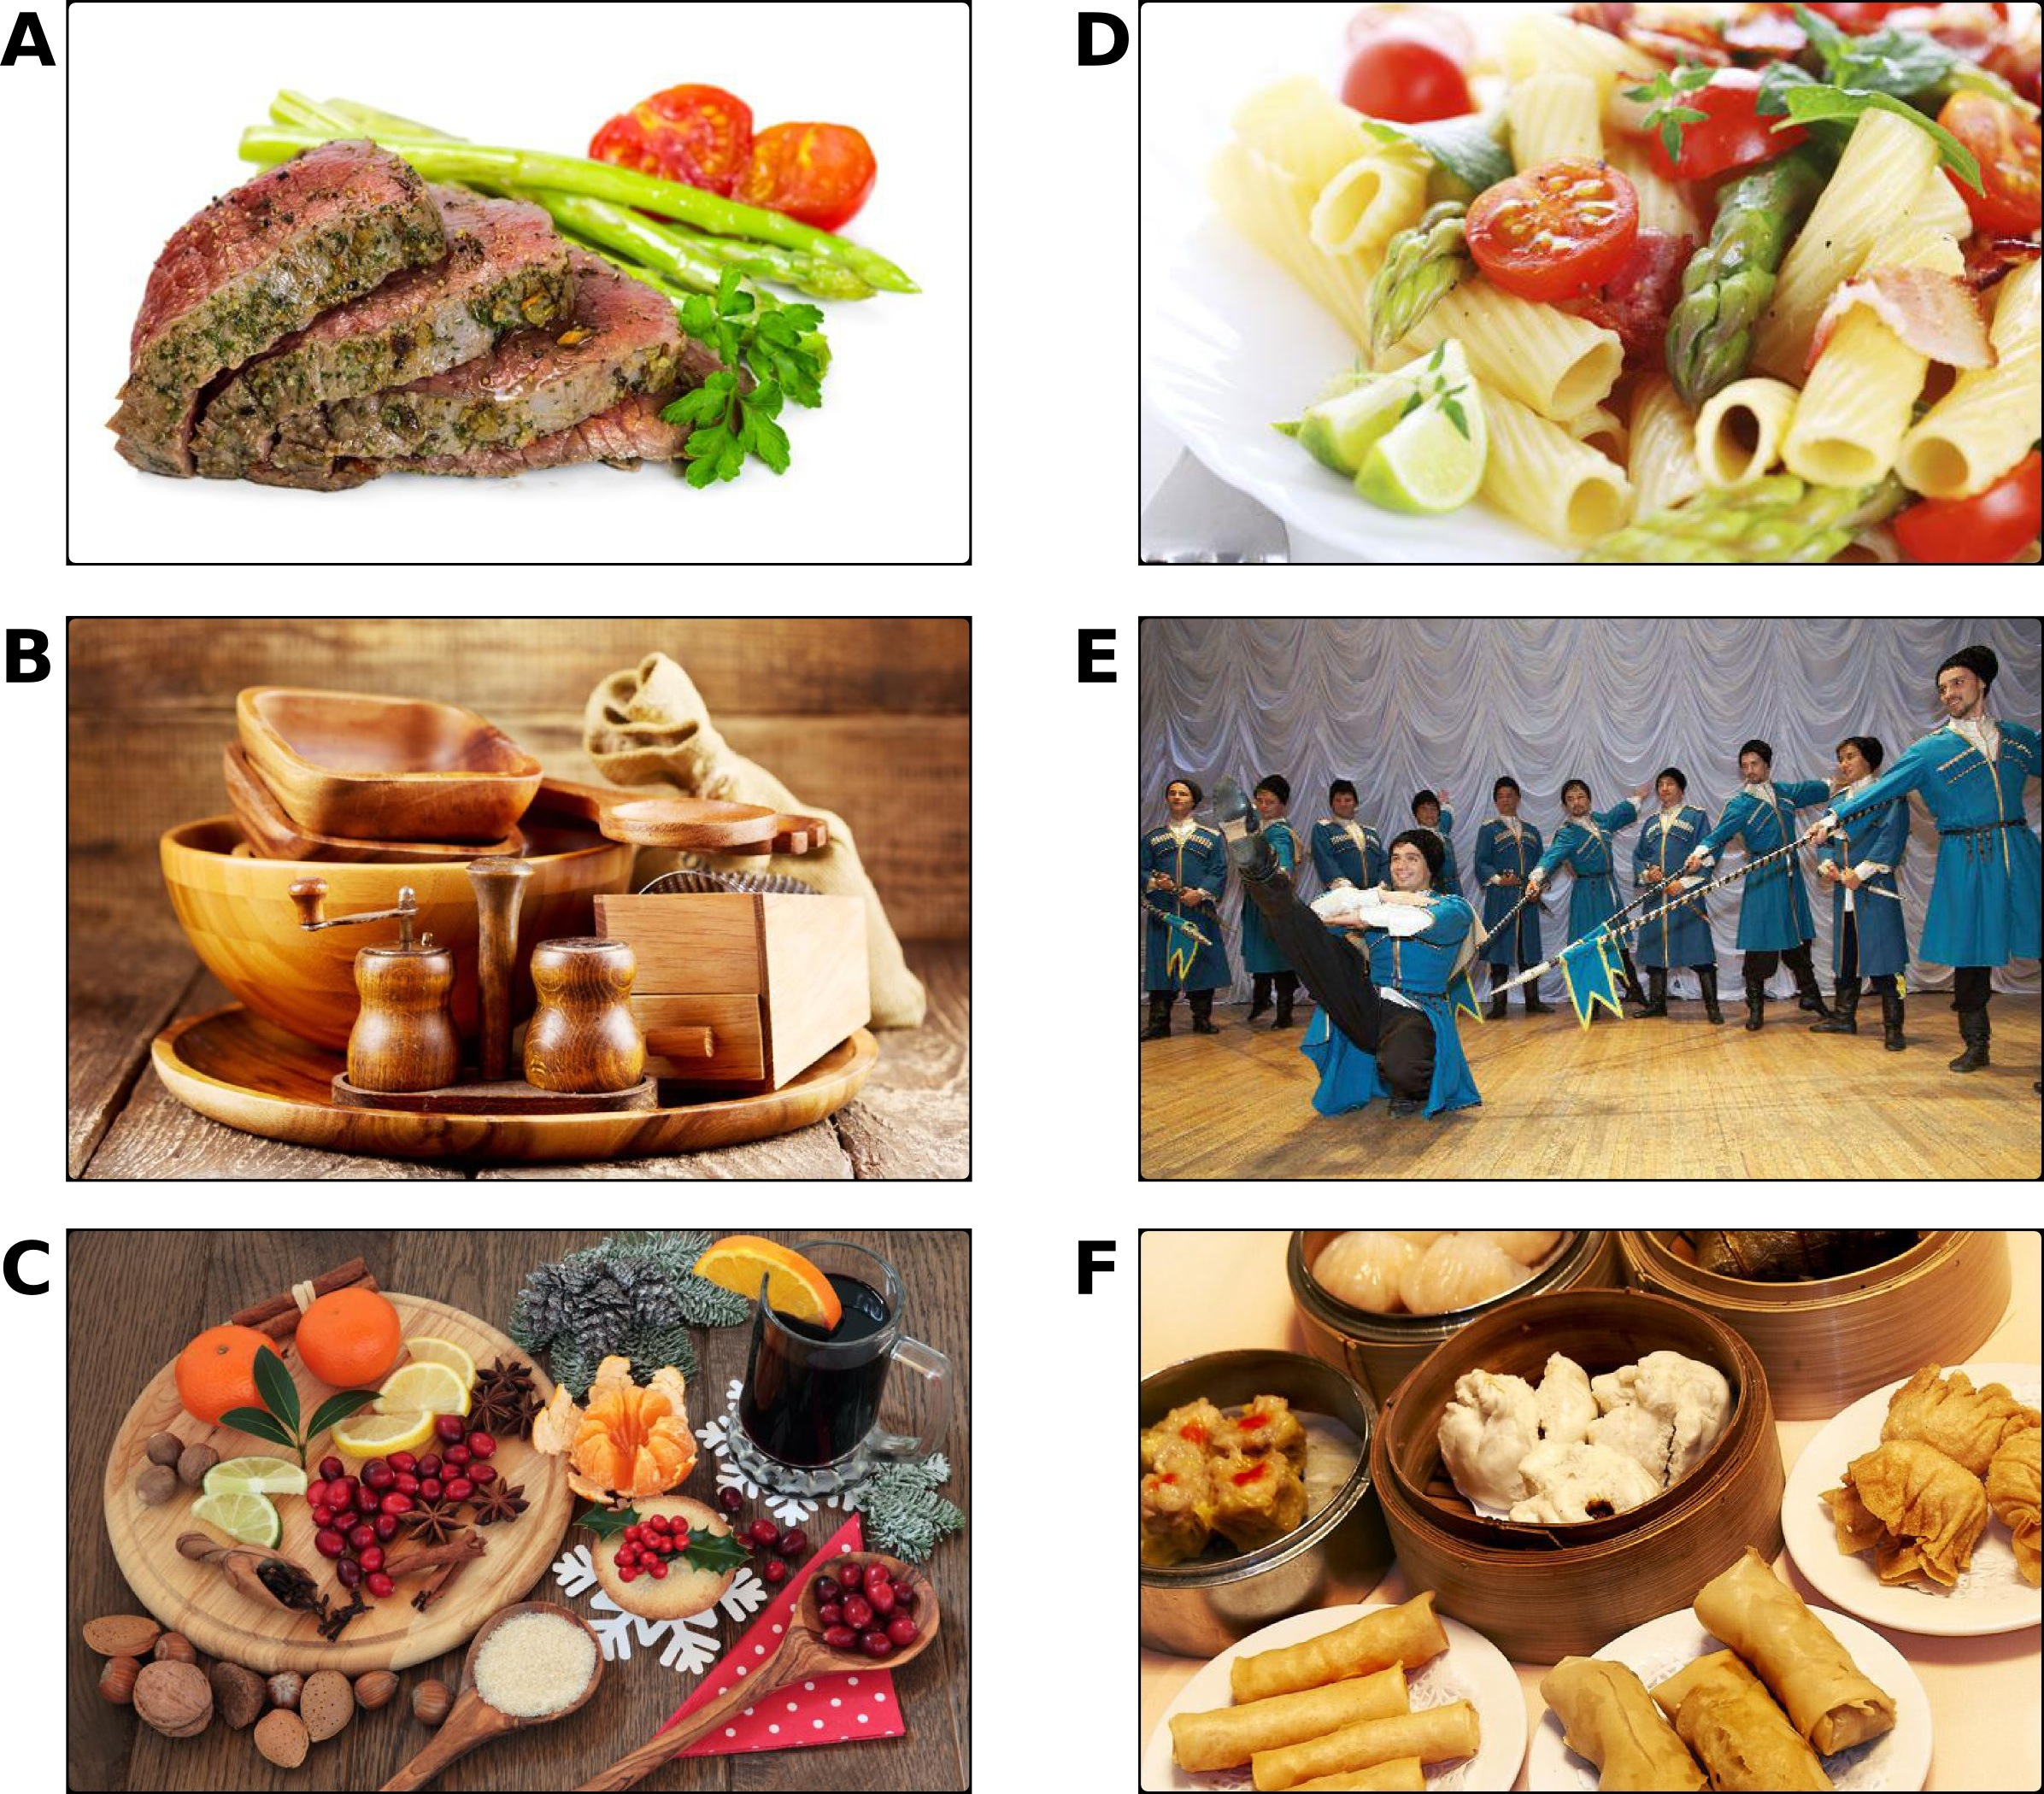
\includegraphics[scale=0.6]{figs/images.pdf}
	\caption{
		Examples of images used in
		initial tasks for the (\textbf{A}) \textit{food} and (\textbf{B}) 
		\textit{objects} treatments of \textit{intertask-food-objects};
		(\textbf{C}) test tasks for \textit{intertask-food-objects} and 
		\textit{frame-food-objects};
		initial tasks for the (\textbf{D}) \textit{food} and (\textbf{E}) 
		\textit{culture} treatments of \textit{intertask-food-culture};
		and (\textbf{F}) test tasks for \textit{intertask-food-culture} and 
		\textit{frame-food-culture}.
		The full set of experimental materials is shown in the 
		supplementary text.
	}

	\label{fig:task}
\end{figure}

Using a na\"ive Bayes classifier\footnote{
	We believe na\"ive Bayes is the best choice in this setting, as discussed
	in the supplementary material, and we show results when a support vector
	machine is used instead. 
	We also discuss data preprocessing and show results for alternatives.
}, we found that intertask effects 
lead to a 30\% bias between workers from the \textit{food} and 
\textit{objects} treatments (Fig.~\ref{fig:theta}A).  
This represents a substantial potential to distort microtask data.

There has been considerable interest in the effects that framing can have
on microtask responses
\cite{Kinnaird2012281,chandler2013breaking,thibodeau2013natural}, so,
as a point of comparison, we performed a similar experiment 
in which we framed the purpose of the tasks.  In the experiment 
\textit{frame-food-objects}, workers were either told that 
the tasks were ``Funded by the laboratory for the visual perception of Food 
and Ingredients'', or ``\ldots of Objects and Tools''.  
Framing did induce changes in the frequencies of 
word usage at significance (as determined by $\chi^2$ test; $p=0.0012$), but 
the \textit{extent} of framing-induced bias was not statistically 
distinguishable from zero ($p =0.37$) (Fig.~\ref{fig:theta}A), and was
weaker than the bias due to intertask effects ($p=2.1\times 10^{-5}$).

To assess the permenance of intertask effects, we replicated the experiment
\textit{intertask-food-objects} five times, each time using a different 
permutation of the test tasks.  This enabled us to measure the severity
of bias as a function of task position, independant of the content
of the test task.  We found that bias was strongest for the first test task
(about 28\%), but remained significant through all five test tasks 
($\alpha=0.05$) sustaining over 12\% bias (Fig. \ref{fig:theta}B).

We conducted variants of these experiments using different images, to see 
whether this trend was robust.  In the experiment 
\textit{intertask-food-culture},
workers were either assigned to a \textit{food} or \textit{culture} treatment.
As before, the initial tasks for the \textit{food} treatment contained images 
depicting food (Fig.~\ref{fig:task}D). 
In the \textit{culture} treatment, 
the initial tasks contained images depicting cultural scenes 
(of dance, sport, or music) (Fig.~\ref{fig:task}E).  The test tasks, which were identical for both
treatments, included images depicting meals of identifiable cultural 
origin\footnote{
	Despite efforts to the contrary, initial tasks 
	in \textit{intertask-food-culture} are arguably still of
	identifiable cultural origin, but this would only tend to make our 
	results more conservative (we discuss this further in the supplementary 
	text).
}
(Fig.~\ref{fig:task}F).  

Results for this experiment again showed a 
strong bias as a result of intertask effects (about 50\%) 
(Fig.~\ref{fig:theta}A).  Again, we compared intertask effects to 
framing, by performing an experiment (\textit{frame-food-culture}) using 
the same test tasks as in \textit{intertask-food-culture}, in which we exposed
workers to a statement framing the purpose of the tasks as the recognition 
of either food or culture.  
In this experiment, framing did not induce significant changes in the 
frequencies of words used during test tasks (by $\chi^2$ test, $p=0.29$) 
(Fig.~\ref{fig:theta}A).

It was only when we combined the use of framing, with an active 
reiteration step, that bias reached a level comparable to that achieved 
by intertask effects.  In the experiment \textit{echo-food-objects},
after framing the purpose of the task around either the recognition of food
or objects, we required the worker to echo back the purpose of the task
using a combo-box input.  In this case, workers exposed to different 
``echoed framing'' showed a bias of about 35\% in the labels provided during 
test tasks
(Fig.~\ref{fig:theta}A). However, it is difficult to say whether this 
should be considered as a framing treatment \textit{per se}.
Requiring the worker to reiterate the frame signals our intent, as the 
requester, to ensure that the worker has taken note of the framing statement, 
possibly leading the worker to interpret it as an instruction.  
In any case, it is remarkable that intertask effects
were on par with an explicit statement of purpose that was emphasized 
through reiteration.

\begin{figure}
	\centering
	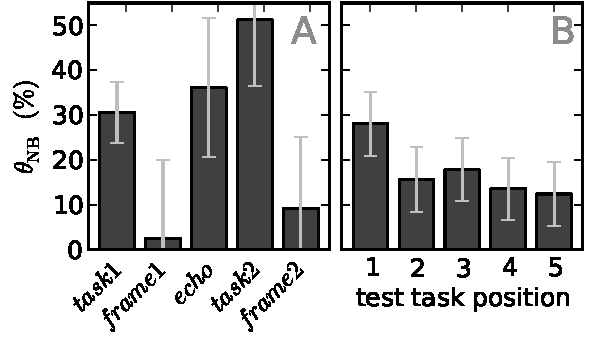
\includegraphics[scale=1]{figs/theta.pdf}
	\caption{
		Empirical bias, $\theta_\mathrm{NB}$, measured using a na\"ive Bayes 
		classifier, induced in image labeling tasks,
		(\textbf{A}) by exposing workers to initial tasks or framing. 
		As workers proceed through test tasks, the effects of initial tasks 
		wane, as shown (\textbf{B}) for \textit{intertask-food-objects}, but 
		remain significant even after five tasks.  Standard error bars are 
		shown.
	}
	\label{fig:theta}
\end{figure}

\begin{figure}
	\centering
	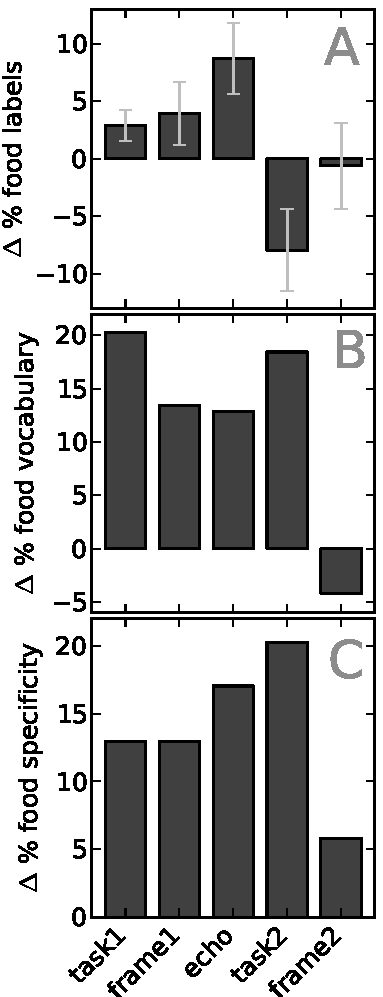
\includegraphics[scale=0.92]{figs/vocab_specificity.pdf}
	\caption{
		(\textbf{A}) Exposing workers to initial tasks or framing, 
		involving food, changed the subsequent fraction of words that 
		referred to food during test tasks, 
		but did not always increase that fraction (in all three plots,
		positive values indicate a larger quantity for food-exposed workers).
		(\textbf{B}) The number of unique food-related
		words (richness) was greater for food-exposed workers, except in the 
		case of \textit{frame-food-culture} (stars indicate the threshold
		for a significant deviation under the null hypothesis of equal 
		richness, $\alpha=0.05$). 
		(\textbf{C}) Food-exposed
		workers used more specialized words to refer to food (see 
		supplementary text for calculation of relative specialization).
		Standard error bars are shown in (\textbf{A} and \textbf{C}).
	}
	\label{fig:specificity}
\end{figure}

To better understand the nature of 
intertask effects, we investigated the vocabulary
that workers used to label test tasks. A natural expectation is that, during
the test tasks within
a given experiment, the food-primed workers would use food-related words 
more often than their non-food-primed counterparts.  However, this was not 
generally 
the case. In the \textit{intertask-food-culture} experiment, food-primed
workers actually used significantly \textit{fewer} food-related words 
during test tasks\footnote{
	food-related words were identified using the wordnet corpus, 
	augmented with additional words obtained by crawling a recipe website 
	(see supplementary text for details).
} (Fig.~\ref{fig:specificity}A).  This finding
rules out a seemingly-simple idea that workers emphasize
content that has been present in earlier tasks: seeing content in prior tasks
influences, but does not necessarily \textit{increase}, the probability of 
referring to the content in subsequent tasks.

To deepen our understanding, we investigated workers' lexical richness in 
reference to food, that is, the number of \textit{unique} food-related words
used.  Even if workers provide an abundance of food-related words, there
can be less diversity if the same words are often repeated.  
This could happen, for example, if workers use generic references 
to food.
Both \textit{intertask} experiments showed that food-exposed workers had 
greater lexical richness, in reference to food, than their non-food-primed 
counterparts (as much as 20\% more) (Fig.~\ref{fig:specificity}B).  
The increase in lexical richness in the case of 
\textit{intertask-food-culture} is particularly noteworthy, because in that 
experiment, food-primed workers made fewer total references to food.  
We also observed enrichment of the food-related lexicon in the 
\textit{priming-food-objects}, and \textit{echo-food-objects} experiments, 
although to a lesser extent.

The observations regarding lexical richness lead us to suspect that 
initial tasks might influence workers to use more refined or specialized 
words, when referring to aspects of content that had been present in the 
initial tasks (i.e. food).  This would help explain why, in the case of 
\textit{intertask-food-culture}, we observed a significantly greater 
\textit{diversity} of food-related words despite their significantly lesser 
\textit{total amount}.
To test whether exposure to food in initial tasks increased the specialization
of food-references, we used the wordnet corpus to operationalize the 
notion of word specialization.  Wordnet provides a set of hypernym-hyponym 
relations between 117,798 English nouns 
\cite{miller1995wordnet,felbaum1998wordnet}.  Hypernyms are generalizations 
(for example, ``bread'' is a hypernym for 
``pumpernickel''), while hyponyms are specializations.
For each experiment, we compared food-related words provided by workers from 
one treatment to those from the other, tallying the percent-excess of
cases where one treatment's words were more specialized than the other 
(detailed calculation in the supplementary text). 

In all experiments except \textit{frame-food-culture}, food-primed workers 
used significantly more specialized words, in reference to food, 
than their non-food-primed 
counterparts (about 15\% more) (Fig.~\ref{fig:specificity}C).
It is interesting that such substantial increases in both the lexical 
richness and specialization of food-related words 
held for \textit{intertask-food-culture}, where, as mentioned, we observed 
that food-exposed workers made \textit{fewer} references to food overall. 
These observations point 
to countervailing factors: one factor tending to activate the more 
specialized and less common food-related words 
(yielding greater lexical richness and specialization), and the other tending 
to suppress certain, presumably more common and generic words 
(yielding fewer food-related words in total).

This hypothesis is corroborated when we look at those words whose 
frequencies changed the most from one treatment to another 
(Table~S\ref{table:top-words}).  
The word ``food'', which is the most generic possible food-related word, was 
always \textit{suppressed} among food-primed workers.  In fact, 
for all experiments, ``food'' was the \textit{most suppressed} word.

Taken together, our results can be 
explained through a combination of positive and negative priming effects.
Positive priming (usually simply ``priming'') occurs when a prior stimulus 
predisposes a person to give certain responses in an ensuing task, and
is often observed as an increase in the speed or accuracy of a response, or
the ability to recognize briefer or noisier stimuli 
\cite{BJOP1796,BJOP1826,Huber2008324}.
Negative priming occurs when, after exposure to a stimulus 
considered to be non-salient, subsequent recognition of the stimulus is 
inhibited \cite{mayr2007negative}.

Workers exposed to images containing food will be (positively) primed, 
activating memories, concepts, and vocabulary related to food.  
However, as the worker labels successive images containing food, the basic 
fact that an image contains food will not appear to be salient, since it 
does not serve to distinguish one image from another.  Thus, the most 
generic references to that fact, such as the label ``food'', 
will be suppressed, while more specialized references will be elicited.  
Meanwhile, the number of references to food overall might increase or 
decrease, depending on the balance of these factors.  

More generally, we are suggesting that, even though workers are not 
instructed to compare tasks in any way, prior tasks form a 
context relative to which workers judge salience.  Thus, due to a combination 
of negative and positive priming, a worker's focus 
in repeated tasks tends to be directed away from generic, shared features, 
toward specific and distinguishing ones.

Prior to this study, little thought appears to have been given to the 
priming effect that a task can have on those tasks that follow. 
But our findings show this is an  
important design consideration.  
A natural response might be simply to randomize 
task ordering, a practice that is commonly employed.  But the sheer extent of 
bias suggests that this will still introduce a significant amount of noise
into the results.  Even chains of two or three similar tasks, which
will not be reliably eliminated in random permutations, could lead
to the levels of bias we observed in our experiments.
It would be preferable to understand intertask
effects in greater depth so that they might be properly controlled.

Our findings suggest that, through careful task engineering,
it might be possible to achieve greater quality and reproducibility
of responses.  
A consistent goal in human computation is the achievement of expert-level
judgments from non-expert workers \cite{kittur2011crowdforge}.  
This has been achieved in some
applications \cite{snow2008cheap,Mortensen20131020,Warby2014385}. 
The distinction between experts and novices can be 
attributed in part to the possession of specialized knowledge and heuristics. 
But to a large degree, this distinction lies in the ability of 
experts to direct their focus toward salient features, while filtering out 
non-salient ones \cite{kellman2009perceptual}.  Using strategic task 
exposure, it might be possible to guide workers' focus and salience 
attribution, enabling expert-level judgment in a wider variety of 
crowdsourced applications.
We anticipate that future work will yield techniques to control intertask 
effects, both to reduce unwanted bias, as well as tune the 
focus, diversity, and specificity of worker responses.

Here we have shown that a severe bias can be introduced into microtask 
responses, simply from the performance of earlier tasks. 
These effects are much stronger than the effects of framing.  
While our findings raise serious concerns about the 
current state of microtask design, they reveal potential opportunities 
for more 
refined control over worker focus and acuity.  Any application that relies
on the repetitive use of human judgment is likely subject to the phenomena
we described here.  Exploring the pitfalls and opportunities posed by
intertask effects is an important direction for future work, 
in the effort to develop performant and reliable methods for human 
computation.
\bibliography{newbib}
\bibliographystyle{Science}


\pagebreak
\section*{Supplementary Material}
\renewcommand{\figurename}{Figure S\!\!}
\renewcommand{\tablename}{Table S\!\!}
\renewcommand{\theequation}{S\arabic{equation}}
\setcounter{figure}{0}
\setcounter{table}{0}
\setcounter{equation}{0}

Microtask platforms are an increasingly popular way to solicit experimental
participants, as well as to annotate large datasets and obtain other 
judgments which are difficult to automate using only a computer.  
Due to the popularity of microtask platforms, there is interest in 
understanding how various task design factors
influence the reliabality of data obtained using microtask platforms.  
Since workers typically perform similar tasks in quick succession, there is
an opportunity for earlier tasks to effectively prime workers, and induce 
bias in the results obtained.
Here we describe in detail experiments presented in the main text, in which
we investigate the effect that prior tasks have on the responses given during
subsequent ones.  

\subsection*{Materials and Methods}

\paragraph{Microtask setup.}

The work presented in the main text consisted of six experiments involving
HITs (bundles of tasks) performed on Amazon's Mechanical Turk platform.  
The flow of events experienced by a worker when participating in this study 
is depicted in Fig.~S\ref{fig:task_schematic}.  
Each experiment was divided into two treatments.  Treatments for a given 
experiment differed with respect to a particular priming modality, which 
served as the independent variable
(as specified in Table~S\ref{table:experiments}).  
The HITs for treatments of the same experiment always involved the same
test tasks (the last five tasks in the HIT),
the results of which served as the dependent variable.
\begin{figure}
	\begin{center}
	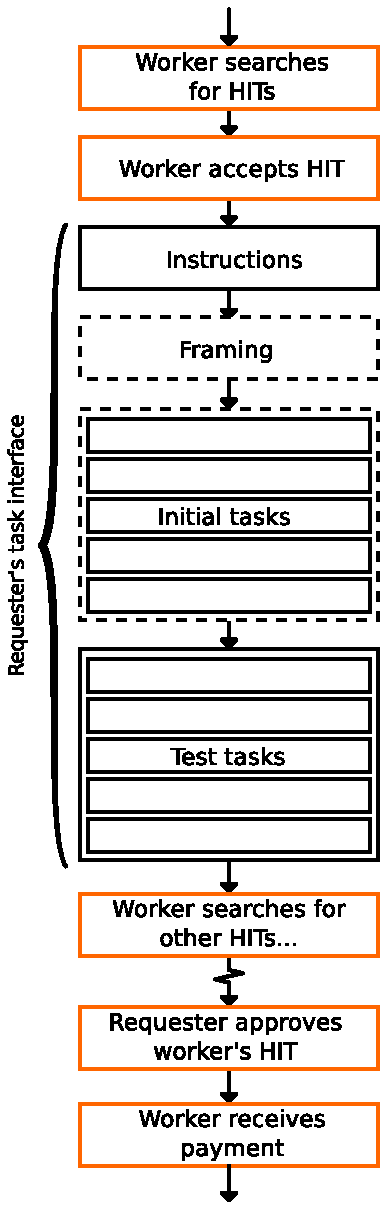
\includegraphics[scale=0.8]{figs/task_schematic.pdf}
	\caption{Flow of events as experienced by a worker participating in
		our study.  Steps with a dash outlined are only performed by 
		workers assigned to certain treatments 
		(see Table~S\ref{table:experiments}).  Steps outlined in orange are
		part of Amazon's Mechanical Turk interface, and are common to any 
		microtask performed on that platform.  Steps outlined in black are
		specific to our HIT.
	}
	\label{fig:task_schematic}
	\end{center}
\end{figure}

All HITs were presented as a series of slides.  The first 
slide consisted of a brief set of instructions.  For HITs that included 
framing, a framing statement was shown on a slide immediately after the 
instructions (Fig. S\ref{fig:hit_preamble}B and C).  
Initial tasks, when included, followed next.  The initial tasks consisted of 
a series of five slides, each containing an image-labeling task like the one 
shown in 
Fig.~S\ref{fig:hit_preamble}D.  Finally, for all HITs, five slides were shown
containing test tasks, in the same format as the initial tasks.

\begin{table}
\centering
\setlength{\tabcolsep}{2pt}
\begin{tabular}{c c c c c c}
\toprule
Experiment & \parbox[c]{3.8cm}{\centering{Priming modality}} & Treatment & Frame & 
	Initial tasks & \parbox[c]{2.0cm}{\centering{Test tasks}} \\
\midrule
\multirow{2}{*}{\textit{intertask-food-objects}} 
& \multirow{2}{*}{initial tasks} & \textit{food} & none 
	& Fig.~S\ref{fig:task1:food} 
	& \multirow{2}{*}{Fig.~S\ref{fig:task1:test}\textsuperscript{g}} \\
& & \textit{objects} & none & Fig.~S\ref{fig:task1:obj} & \\

\noalign{\smallskip}
\hdashline
\noalign{\smallskip}

\multirow{2}{*}{\textit{frame-food-objects}} 
& \multirow{2}{*}{framing} & \textit{food} 
	& ``food''\textsuperscript{a}
	& none & \multirow{2}{*}{Fig.~S\ref{fig:task1:test}} \\
& & \textit{objects} 
	& ``objects''\textsuperscript{b}
	& none & \\

\noalign{\smallskip}
\hdashline
\noalign{\smallskip}

\multirow{2}{*}{\textit{echo-food-objects}} 
& \multirow{2}{*}{echoed framing} & \textit{food} 
	& ``food''\textsuperscript{c}
	& none & \multirow{2}{*}{Fig.~S\ref{fig:task1:test}} \\
& & \textit{objects} 
	& ``objects''\textsuperscript{d}
	& none & \\

\noalign{\smallskip}
\hdashline
\noalign{\smallskip}

\multirow{2}{*}{\textit{intertask-food-culture}} 
& \multirow{2}{*}{initial tasks} & \textit{food} 
	& none
	& Fig.~S\ref{fig:task2:food} 
	& \multirow{2}{*}{Fig.~S\ref{fig:task2:test}} \\
& & \textit{culture} 
	& none & Fig.~S\ref{fig:task2:cult} & \\

\noalign{\smallskip}
\hdashline
\noalign{\smallskip}

\multirow{2}{*}{\textit{frame-food-culture}} 
& \multirow{2}{*}{framing} & \textit{food} 
	& ``food''\textsuperscript{e}
	& Fig.~S\ref{fig:frame2:ingr} 
	& \multirow{2}{*}{Fig.~S\ref{fig:task2:test}} \\
& & \textit{culture} 
	& ``culture''\textsuperscript{f} 
	& Fig.~S\ref{fig:frame2:ingr} & \\

\bottomrule
\end{tabular}
\caption{
	Description of experiments performed.  Each experiment had two treatments
	which differed either in the initial tasks shown or the framing used 
	(the priming modality).  
	During echoed framing, the worker had to respond to the framing language
	using a combo box input (Fig.~S\ref{fig:hit_preamble}C).
	\newline\textsuperscript{a} ``Funded by the laboratory for the visual 
		perception of Food and Ingredients''
	\newline\textsuperscript{b} ``Funded by the laboratory for the visual 
		perception of Objects and Tools''
	\newline\textsuperscript{c} ``The purpose of this study is to understand the visual perception of Food and Ingredients''
	\newline\textsuperscript{d} ``The purpose of this study is to understand the visual perception of Objects and Tools''
	\newline\textsuperscript{e} ``This research is proudly funded by The National 
		Foundation for Nutritional Awareness''
	\newline\textsuperscript{f} ``This research is proudly funded by The Global 
		Foundation for the Recognition of Cultures''
	\newline\textsuperscript{g} Both treatments were divided into five 
	sub-treatments having a different permutation of test tasks.
}
\label{table:experiments}
\end{table}

\begin{figure}
	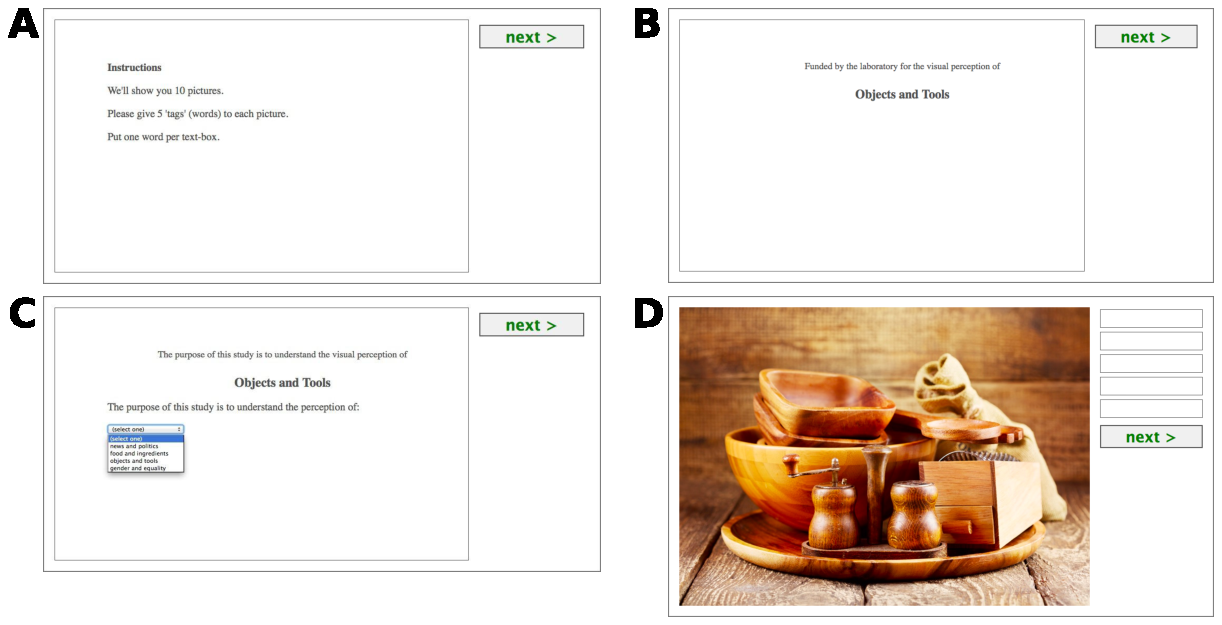
\includegraphics[scale=0.8]{figs/tasks.pdf}
	\caption{Examples of (A) task instructions, (B) a framing slide
		(C) an echoed framing slide, and (D) an image-labeling 
		task.
	}
	\label{fig:hit_preamble}
\end{figure}
Workers were randomly assigned to the treatments, and 
a given worker could only complete one HIT related to this study.  
In \textit{intertask-food-culture}, the \textit{food} and \textit{culture}
treatments were both divided into five sub-treatments, 
in which the test tasks were permuted.  
The permutations were obtained by rotating 
the order shown in Fig.~S\ref{fig:task1:test} by different amounts. 
For example, rotating by one position involves moving the first image to the 
second position, the second image to the third position, and so on, and 
moving the last image to the first position.  
The five different possible rotations were used for the five 
sub-treatments.  This enabled us to study the effects on each image when
it occurred in different positions relative to the initial tasks.

\paragraph{Selection of images.} 

The images used in the initial tasks for \textit{intertask-food-objects}  
are shown in Figs.~S\ref{fig:task1:food} (\textit{food} treatment) and 
S\ref{fig:task1:obj} (\textit{objects} treatment).
We took care to exclude objects from
the food-images (except for the dish supporting the food in some cases), and 
to exclude food from the object-images.  The images used for the test tasks
of \textit{intertask-food-objects} and \textit{frame-food-objects} are shown 
in Fig.~S\ref{fig:task1:test}.

The images used in the initial tasks
for \textit{intertask-food-culture} are shown in Figs.~S\ref{fig:task2:food} 
(\textit{food} treatment) and S\ref{fig:task2:cult} 
(\textit{culture} treatment).
We selected the initial images for the treatments of this experiment to 
respectively reflect depict food and culture.
Naturally, since food is a very
important aspect of culture, pictorial depictions of the two concepts 
cannot be cleanly separated,
and images depicting food inevitably also depict culture.
However, the fact that the images for the initial tasks in the 
\textit{food} treatment 
of \textit{intertask-food-culture} also depict culture
will only tend to make the \textit{food} and \textit{culture}
treatments more similar. 
This would tend to reduce the severity of intertask 
effects, but we nevertheless still observed strong intertask effects.
Thus, the presence of culture in the food-related initial images of 
\textit{intertask-food-culture} does not seem to have been problematic.
The images used in the test tasks of \textit{intertask-food-culture} and
\textit{frame-food-culture} are shown in Fig.~S\ref{fig:task2:test}.

\begin{figure}
	\begin{center}
	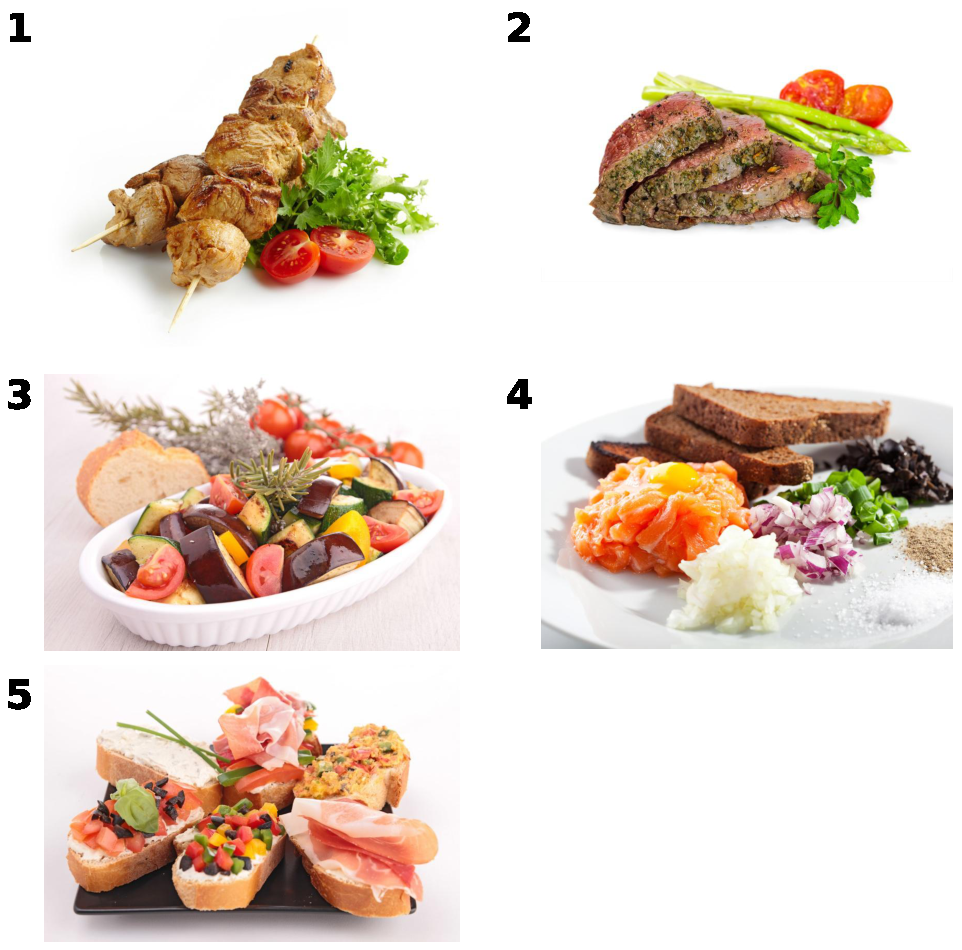
\includegraphics{figs/task1-food.pdf}
	\end{center}
	\caption{
		Images used in the initial tasks for the
		\textit{food} treatment of \textit{intertask-food-objects}.  
		The numbers show the order in which the 
		images were presented to workers.
	}
	\label{fig:task1:food}
\end{figure}

\begin{figure}
	\begin{center}
	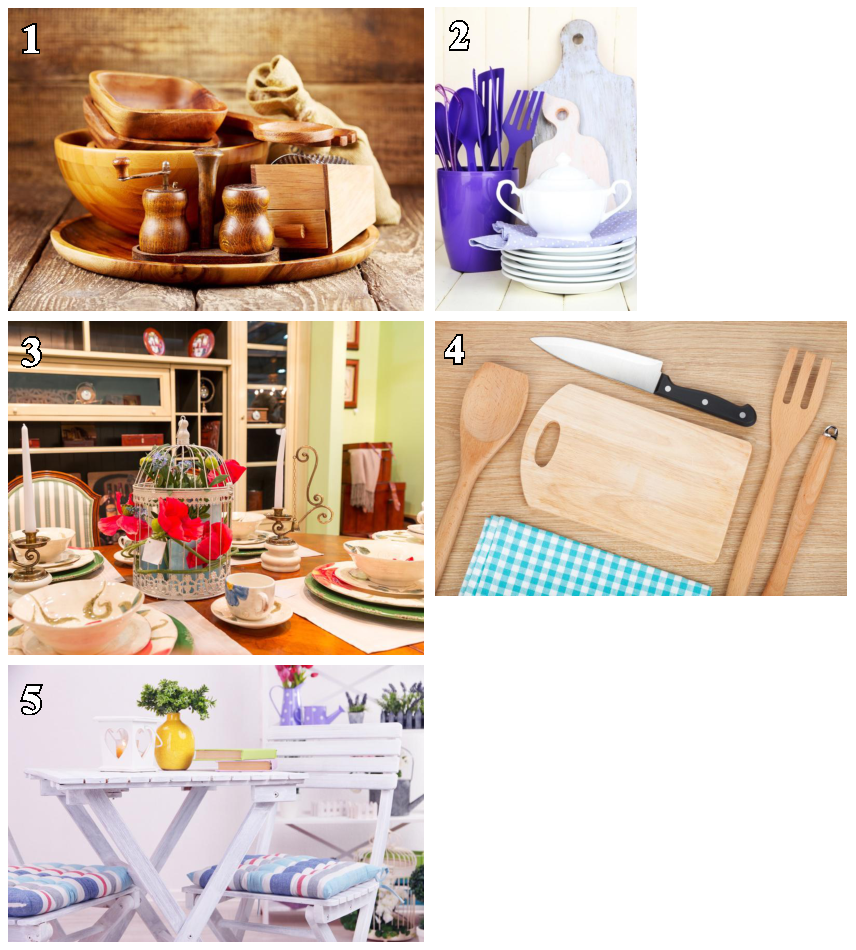
\includegraphics{figs/task1-obj.pdf}
	\end{center}
	\caption{
		Images used in the initial tasks for the
		\textit{objects} treatment of \textit{intertask-food-objects}.  
		The numbers show the order in which the images were presented to 
		workers.
	}
	\label{fig:task1:obj}
\end{figure}

\begin{figure}
	\begin{center}
	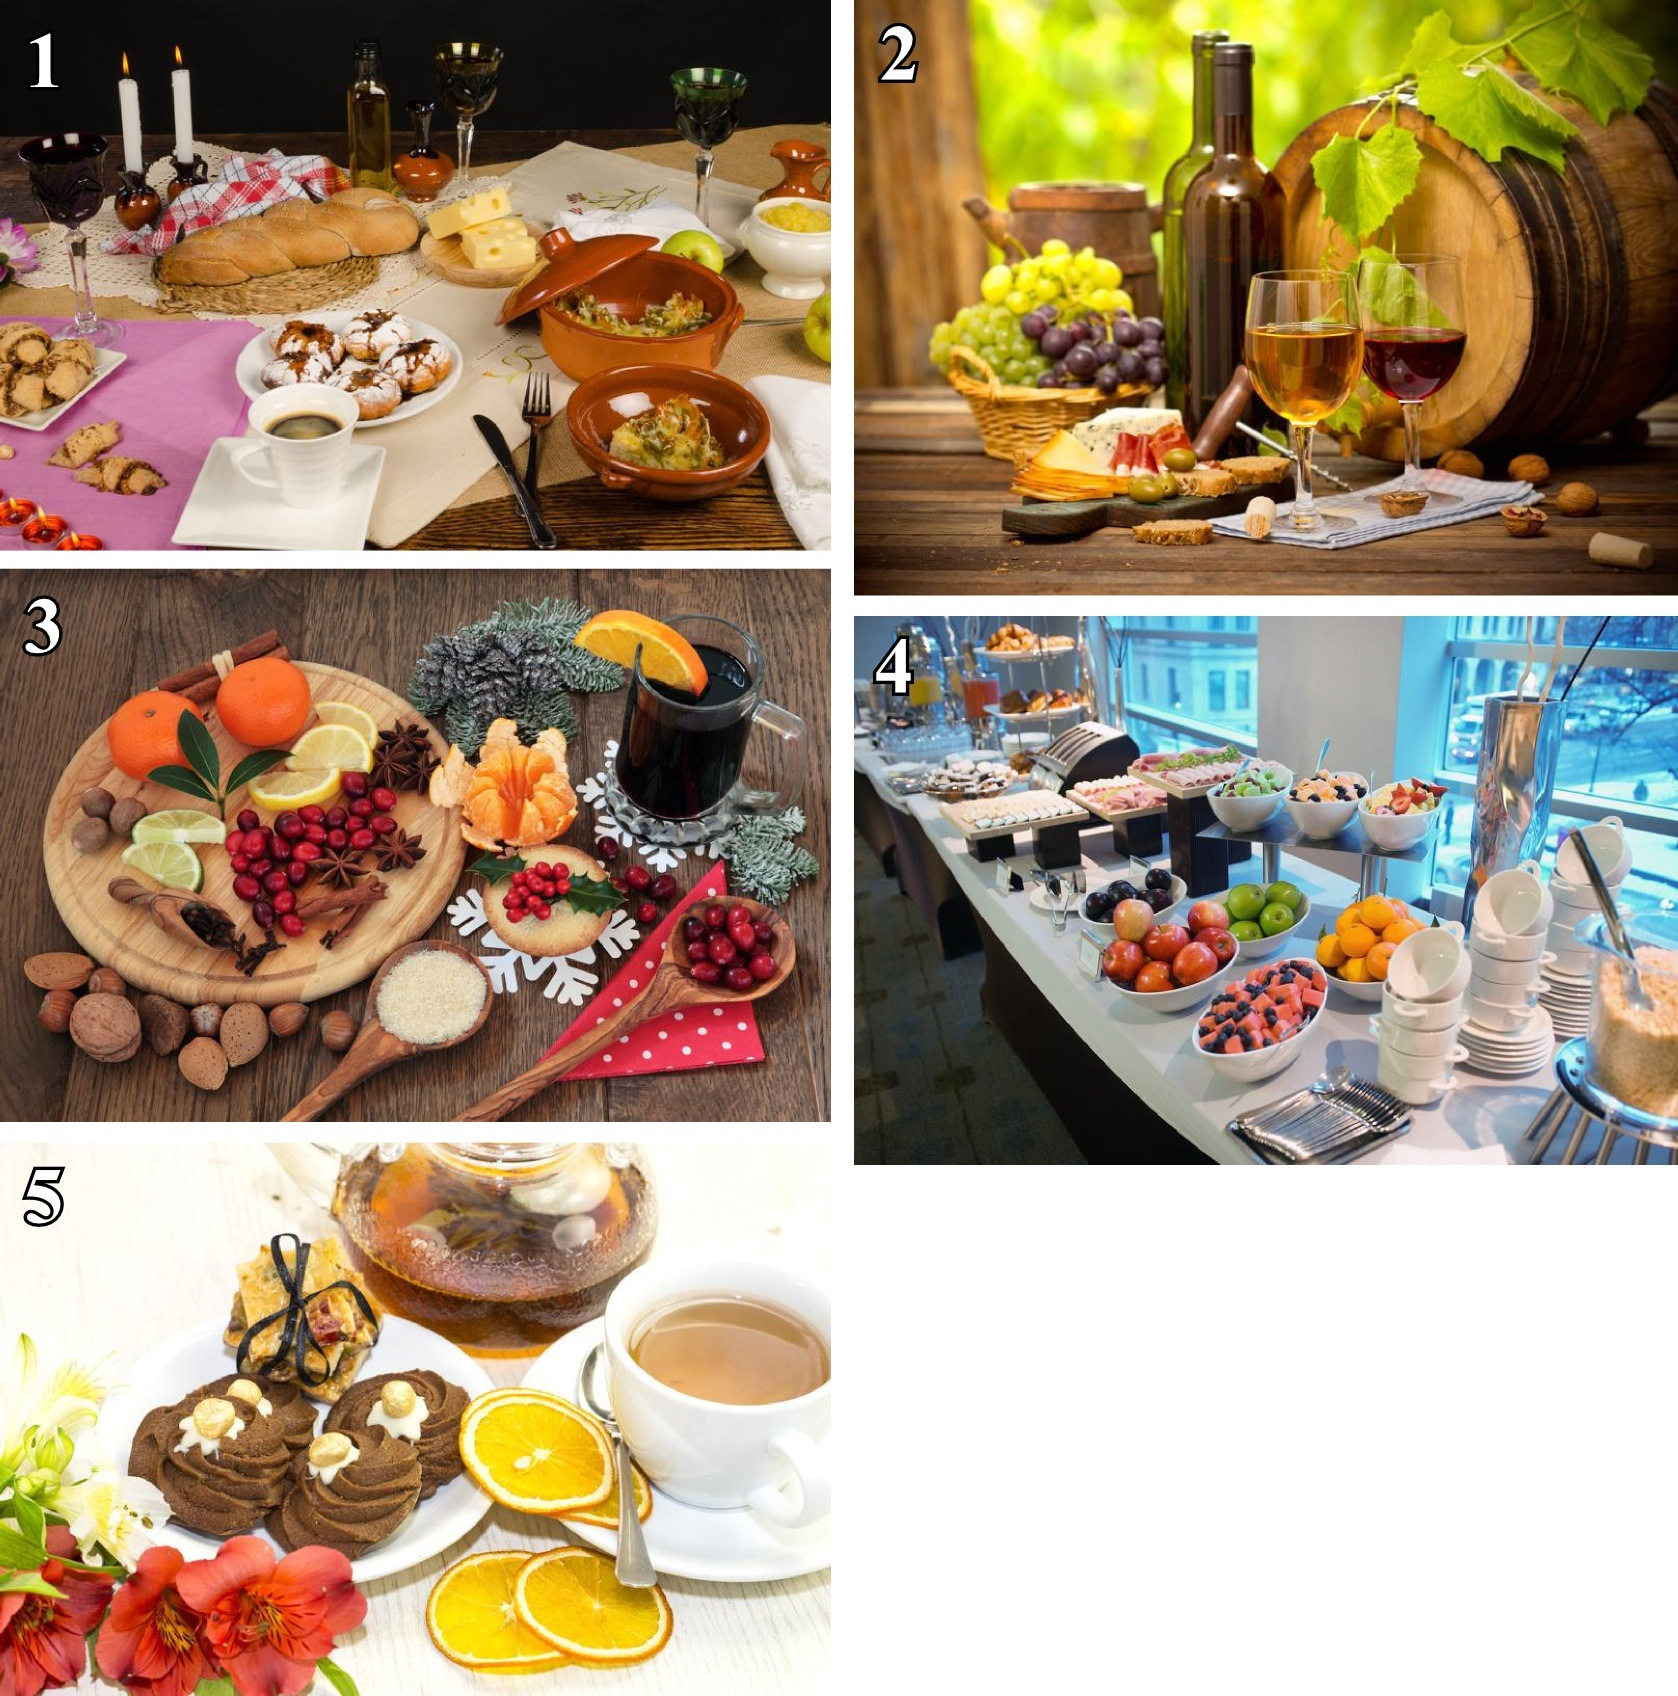
\includegraphics{figs/task1-test.pdf}
	\end{center}
	\caption{
		Images used in the test tasks for \textit{intertask-food-objects}
		and \textit{frame-food-objects}.  
		The numbers show the order in which the 
		images were presented to workers in \textit{frame-food-objects};
		in \textit{intertask-food-objects}, five different orderings were
		used, which can be obtained by taking the numbers shown, $n$,
		and replacing them by $n + c \bmod 5$ for $c$ running from 0 to 4.
	}
	\label{fig:task1:test}
\end{figure}

\begin{figure}
	\begin{center}
	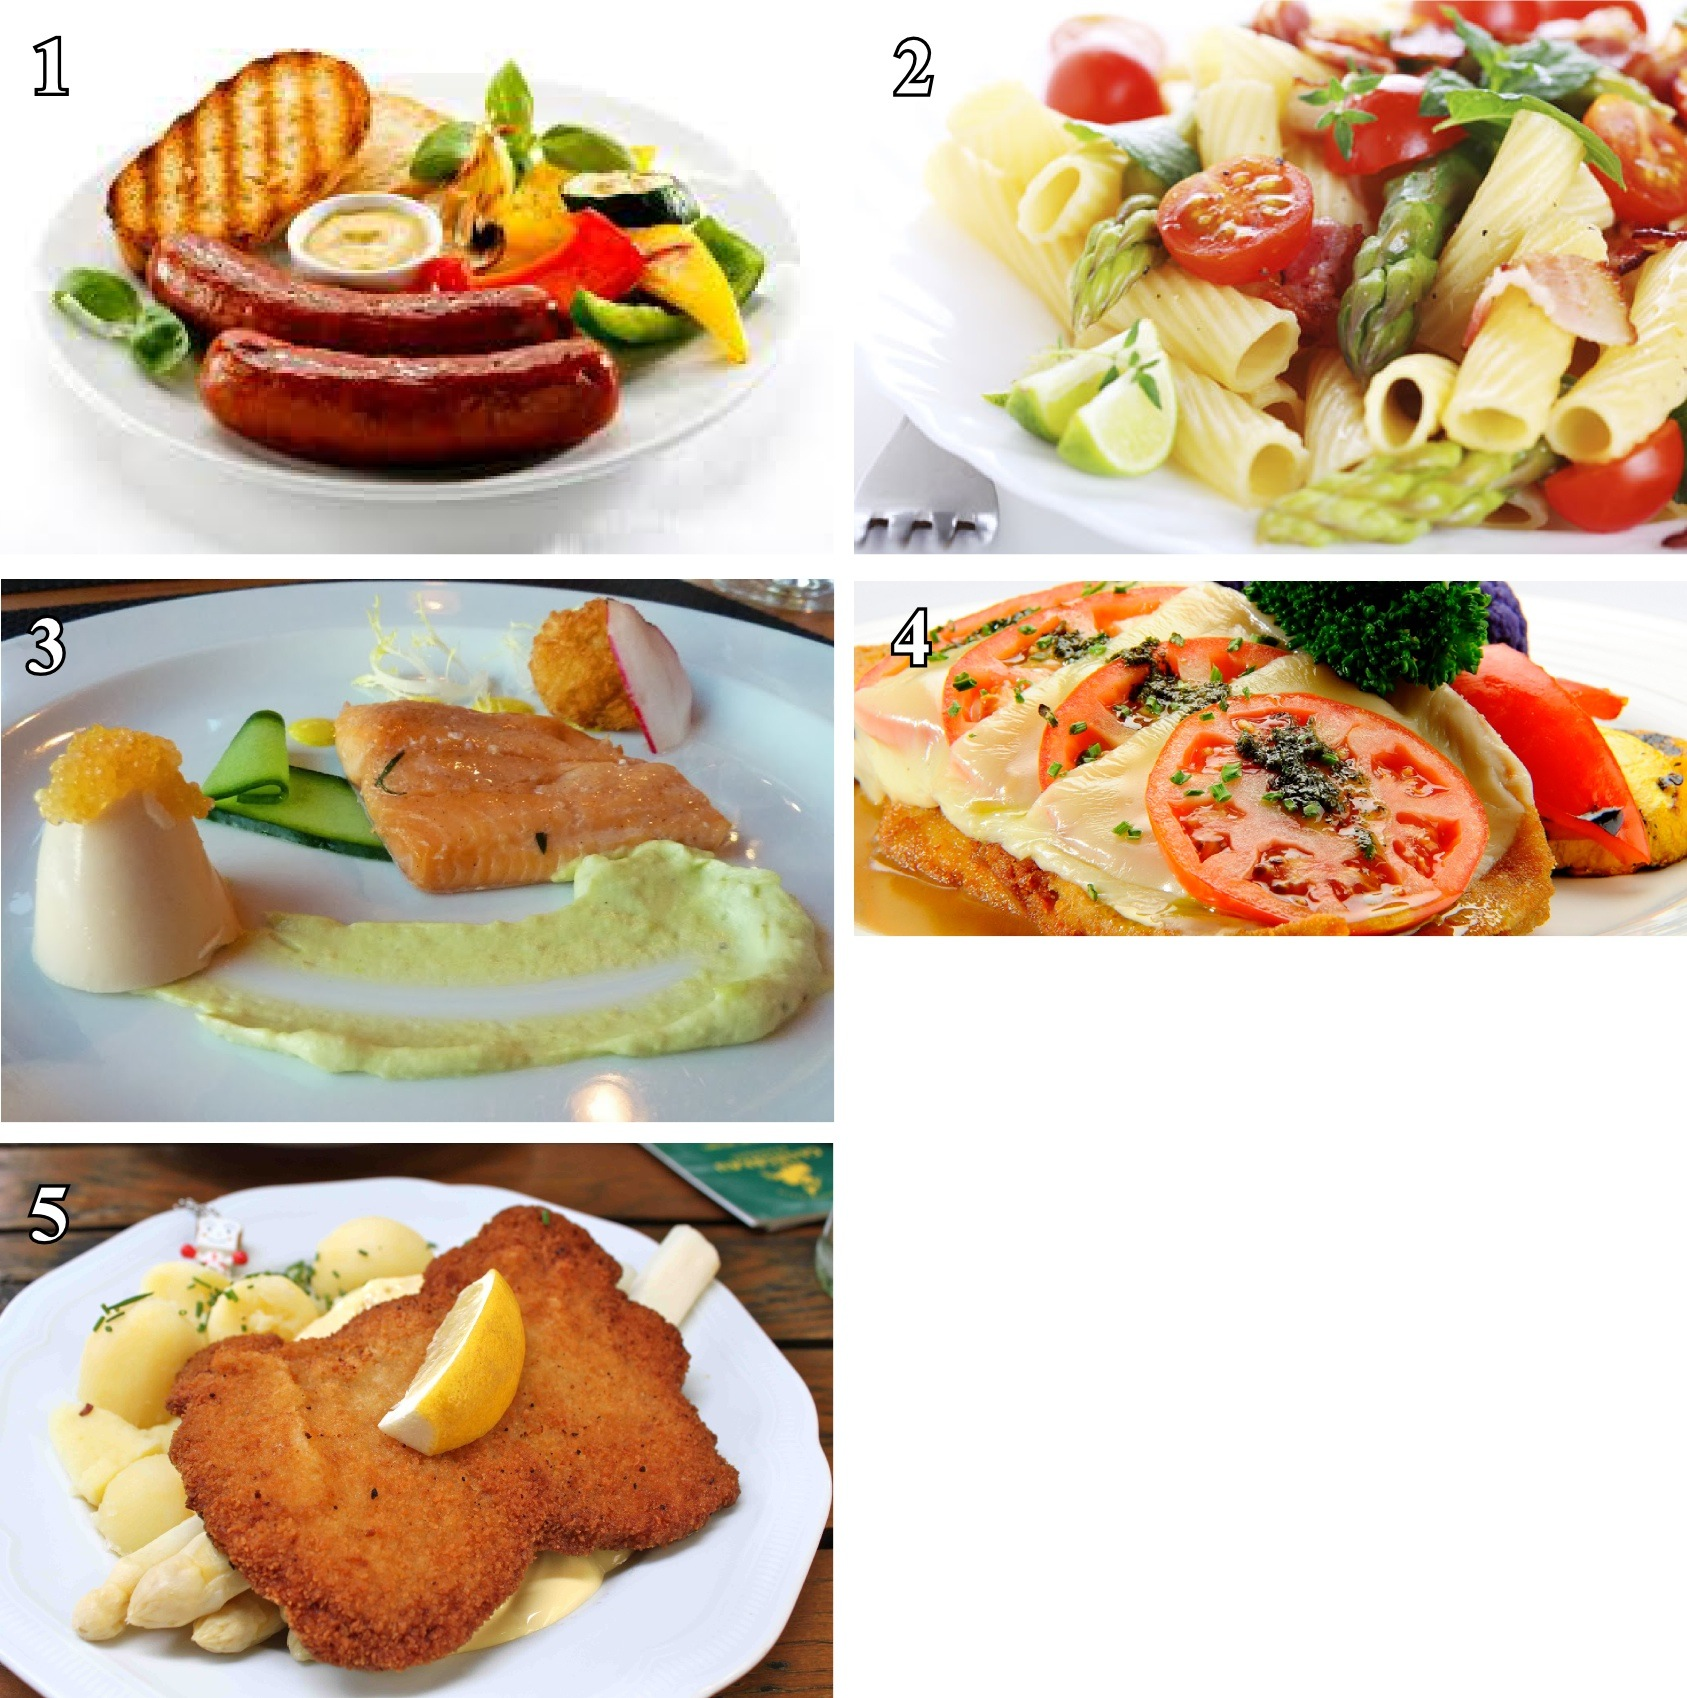
\includegraphics{figs/task2-food.pdf}
	\end{center}
	\caption{
		Images used in the initial tasks for the
		\textit{food} treatment of \textit{intertask-food-culture}.  
		The numbers show the order in which the 
		images were presented to workers.
	}
	\label{fig:task2:food}
\end{figure}

\begin{figure}
	\begin{center}
	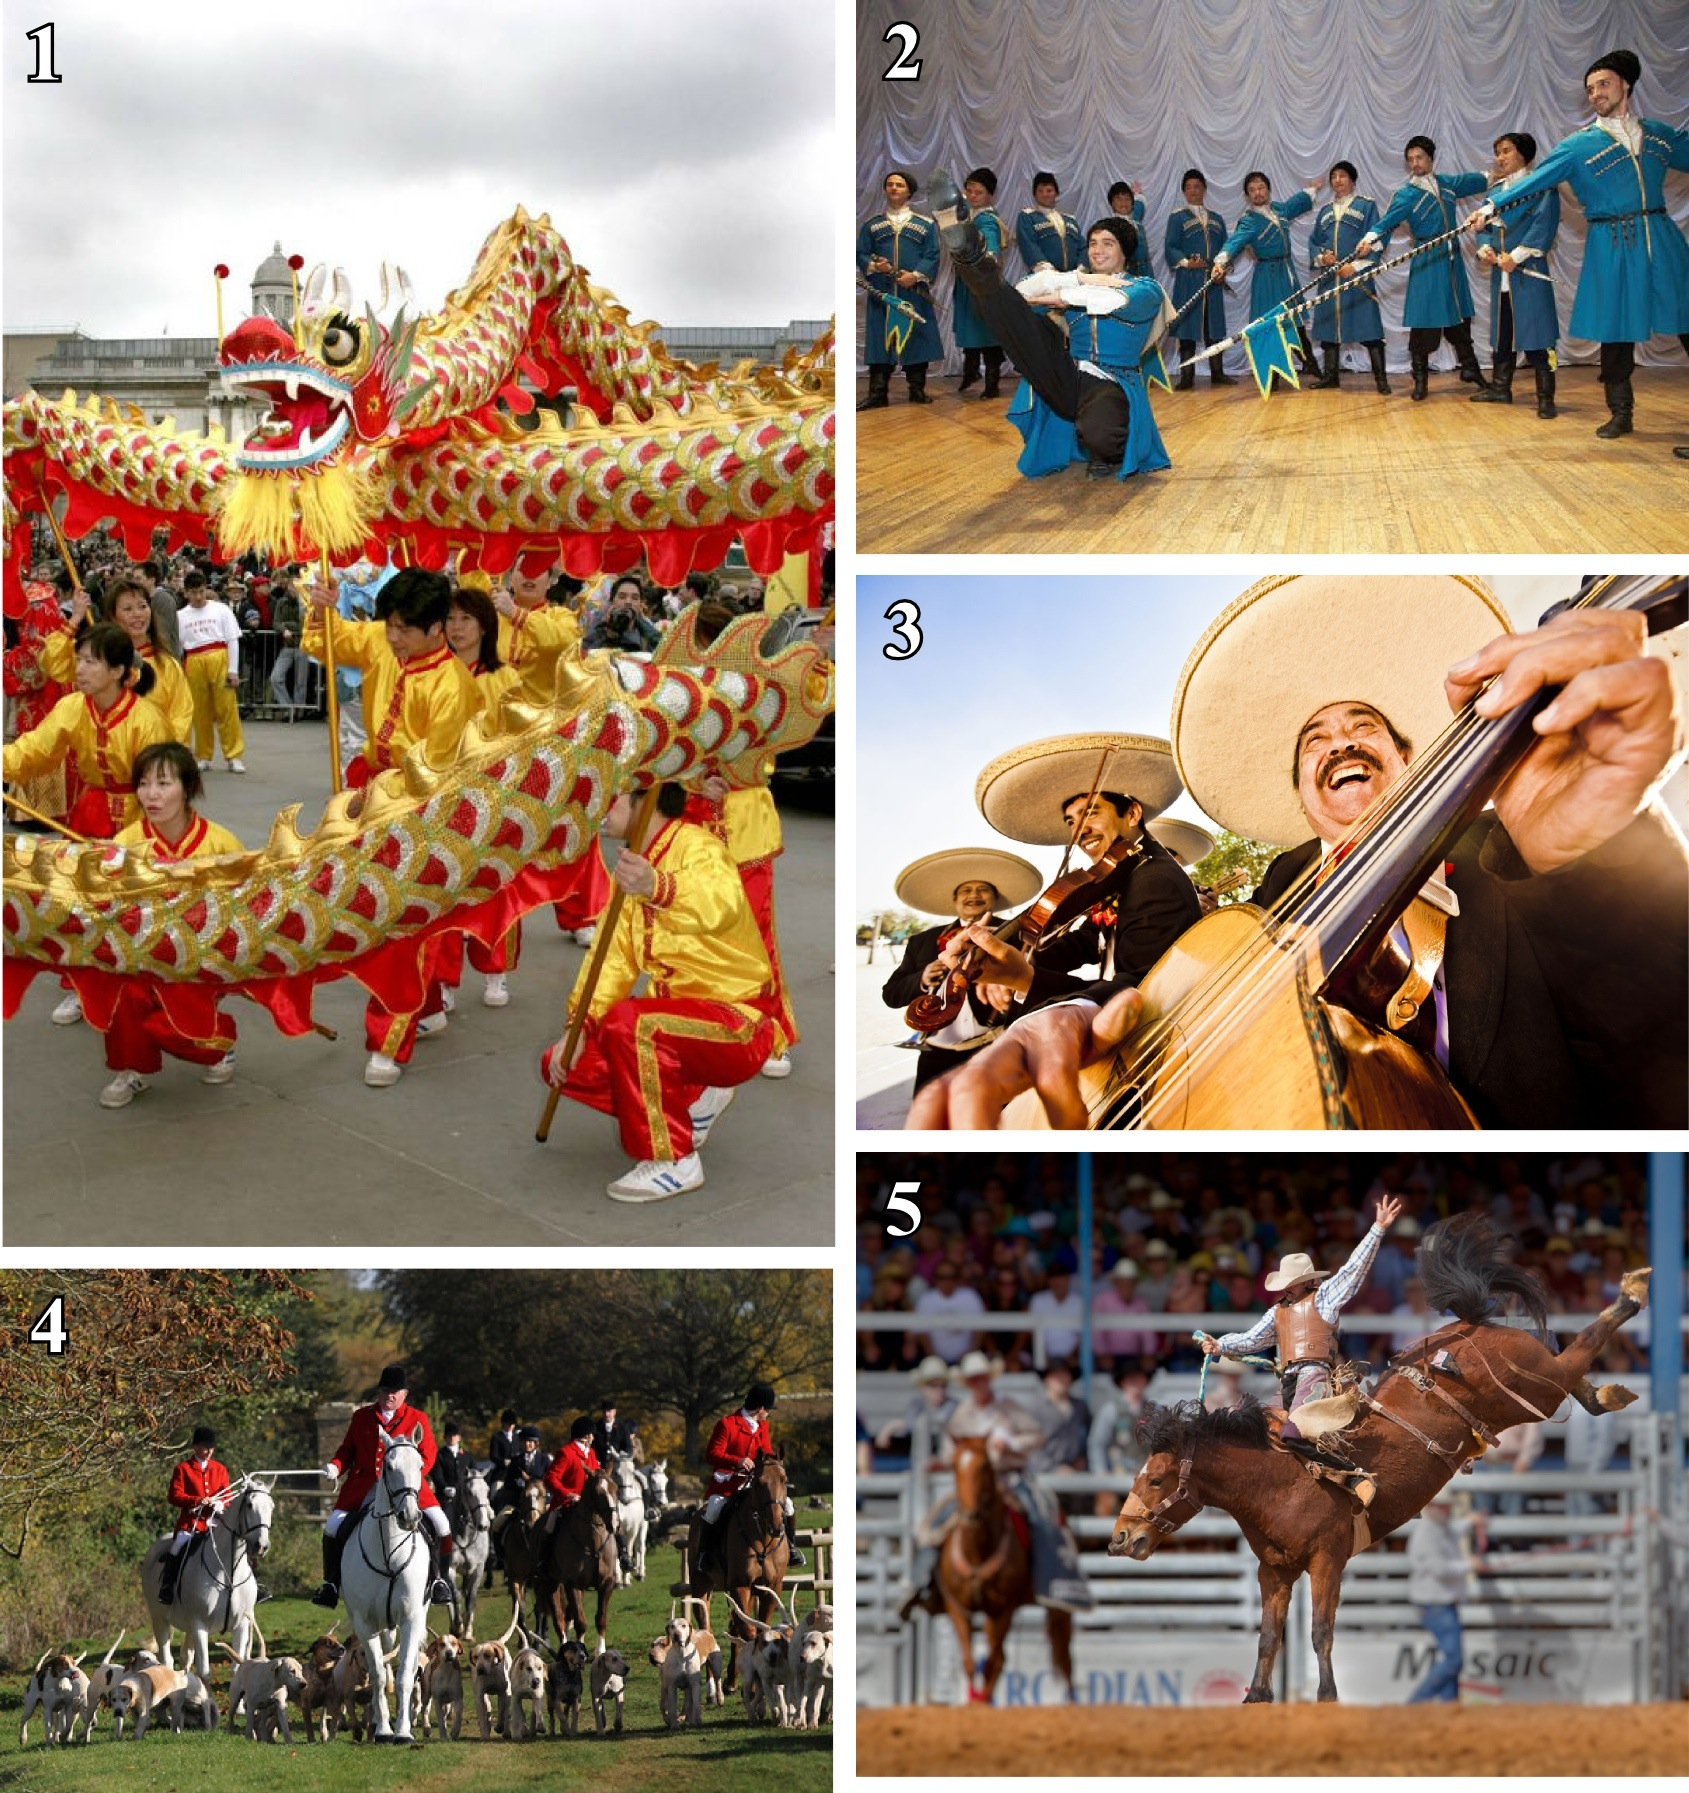
\includegraphics{figs/task2-cult.pdf}
	\end{center}
	\caption{
		Images used in the initial tasks for the
		\textit{culture} treatment of \textit{intertask-food-culture}.  
		The numbers show the order in which the 
		images were presented to workers.
	}
	\label{fig:task2:cult}
\end{figure}

\begin{figure}
	\begin{center}
	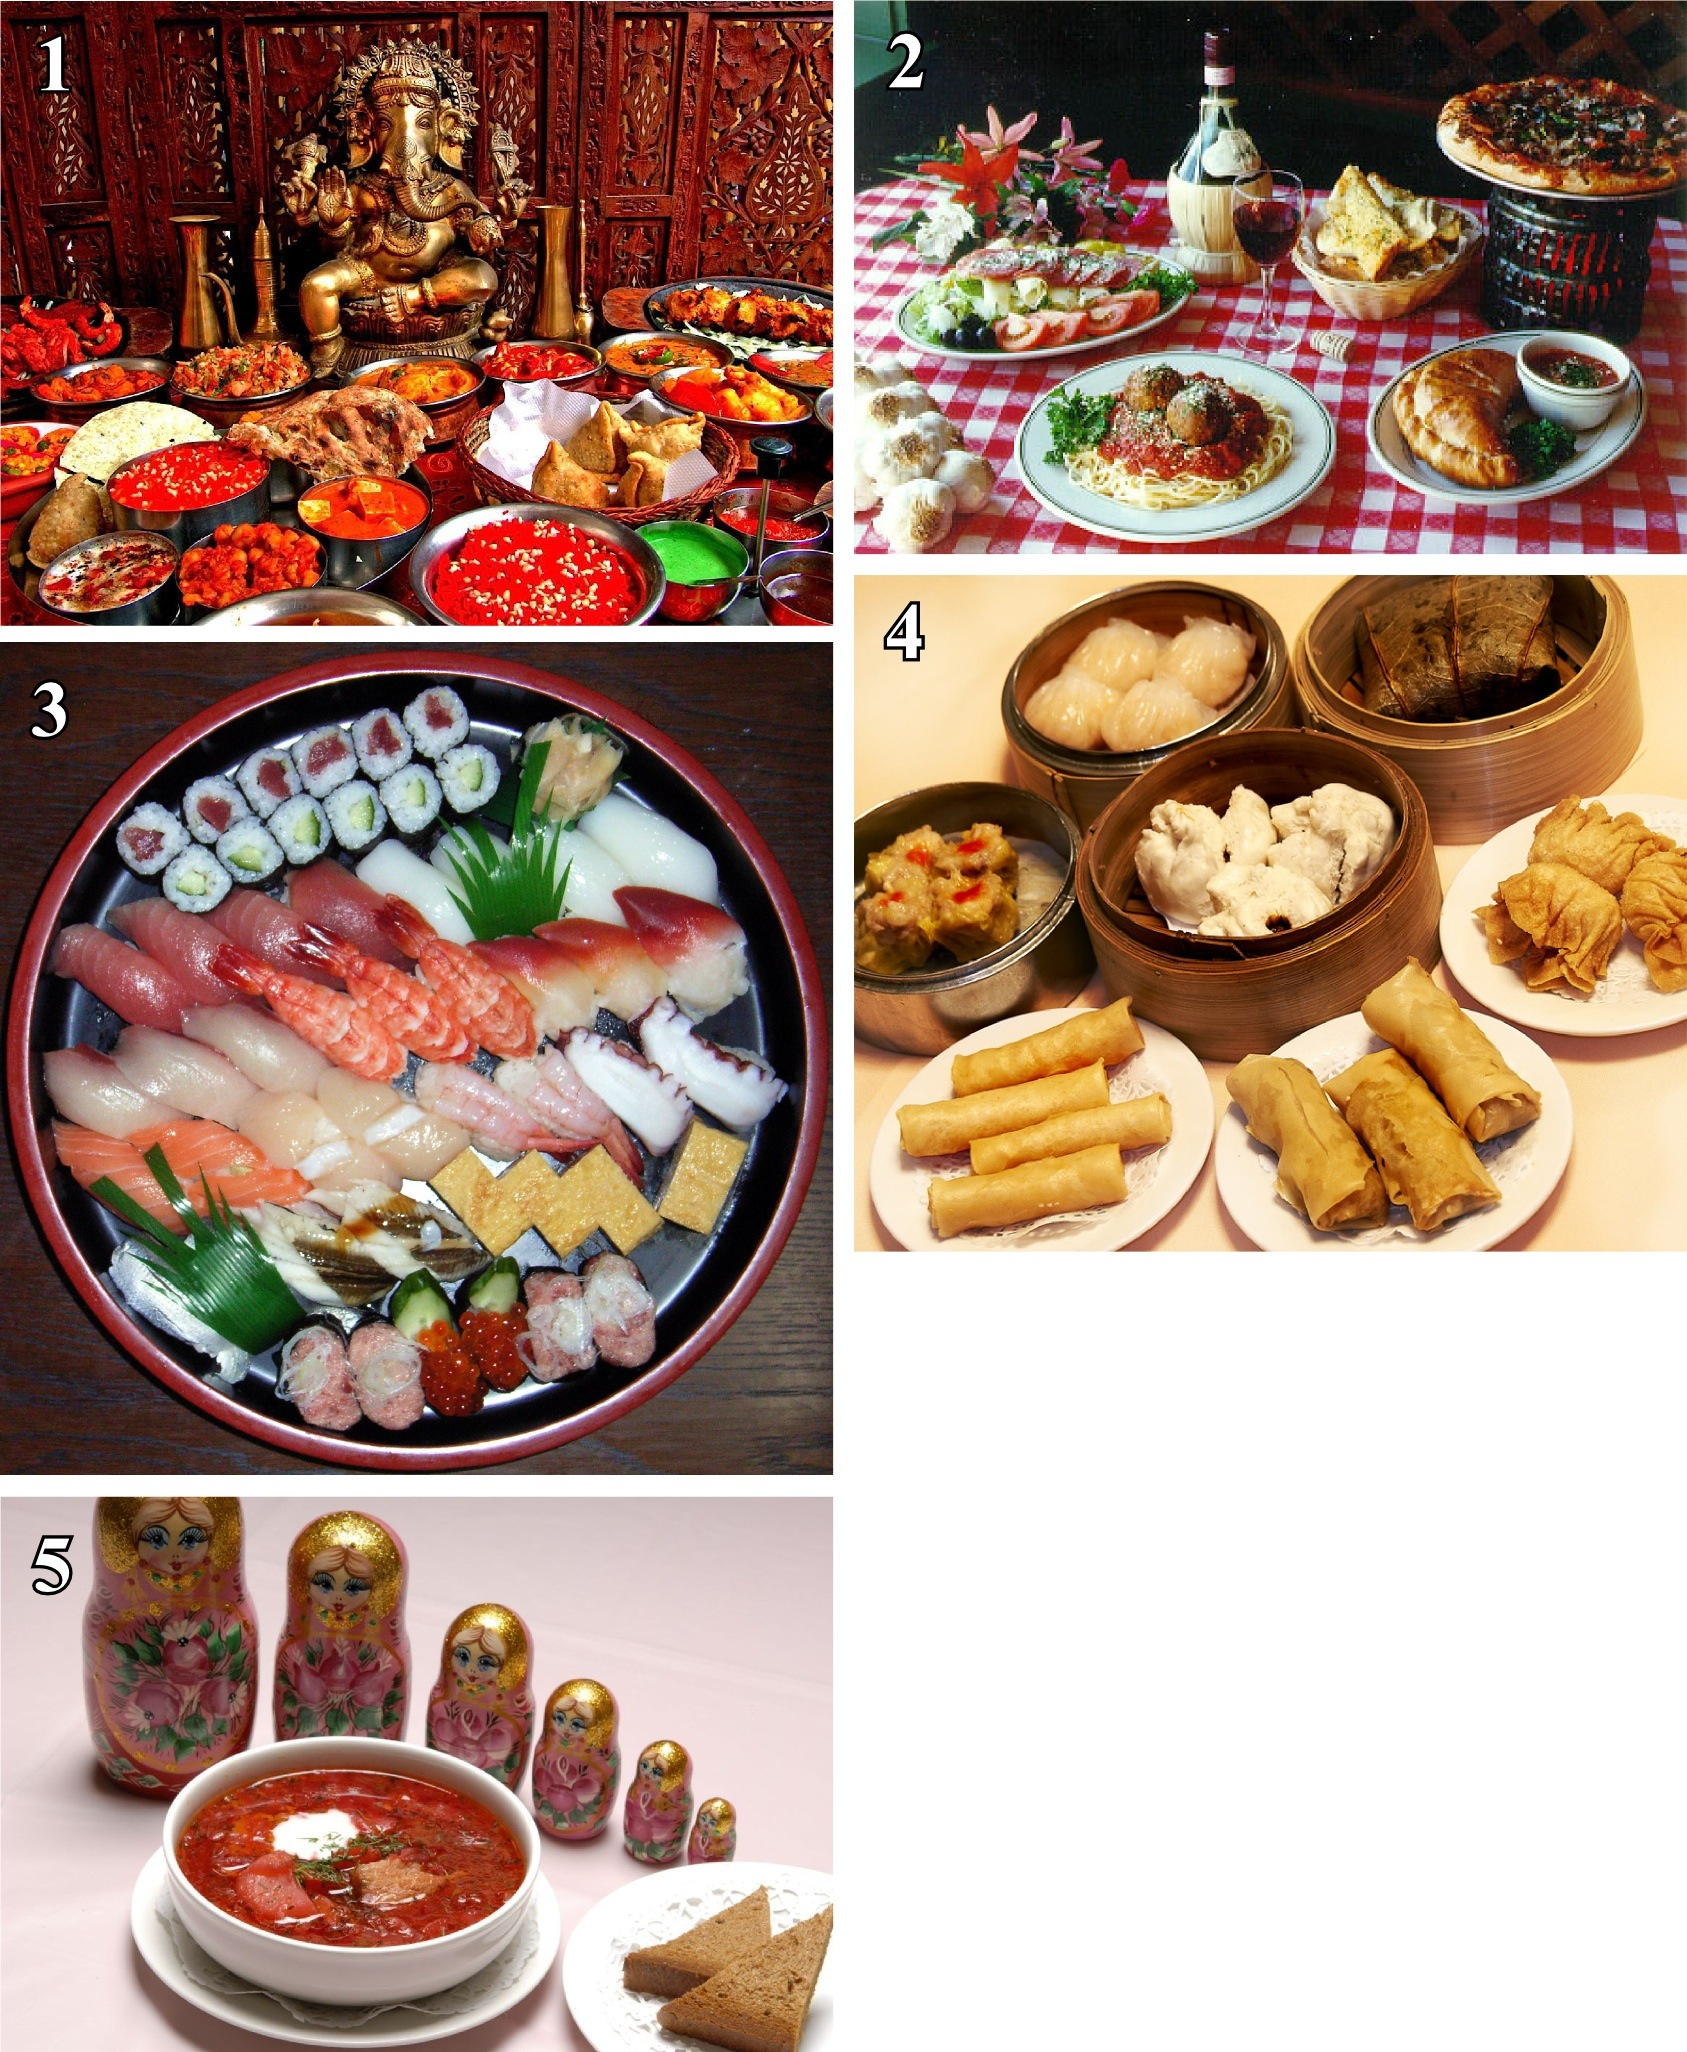
\includegraphics{figs/task2-test.pdf}
	\end{center}
	\caption{
		Images used in the test tasks for \textit{intertask-food-culture} 
		and \textit{frame-food-culture}.  
		The numbers show the order in which the 
		images were presented to workers.
	}
	\label{fig:task2:test}
\end{figure}

\begin{figure}
	\begin{center}
		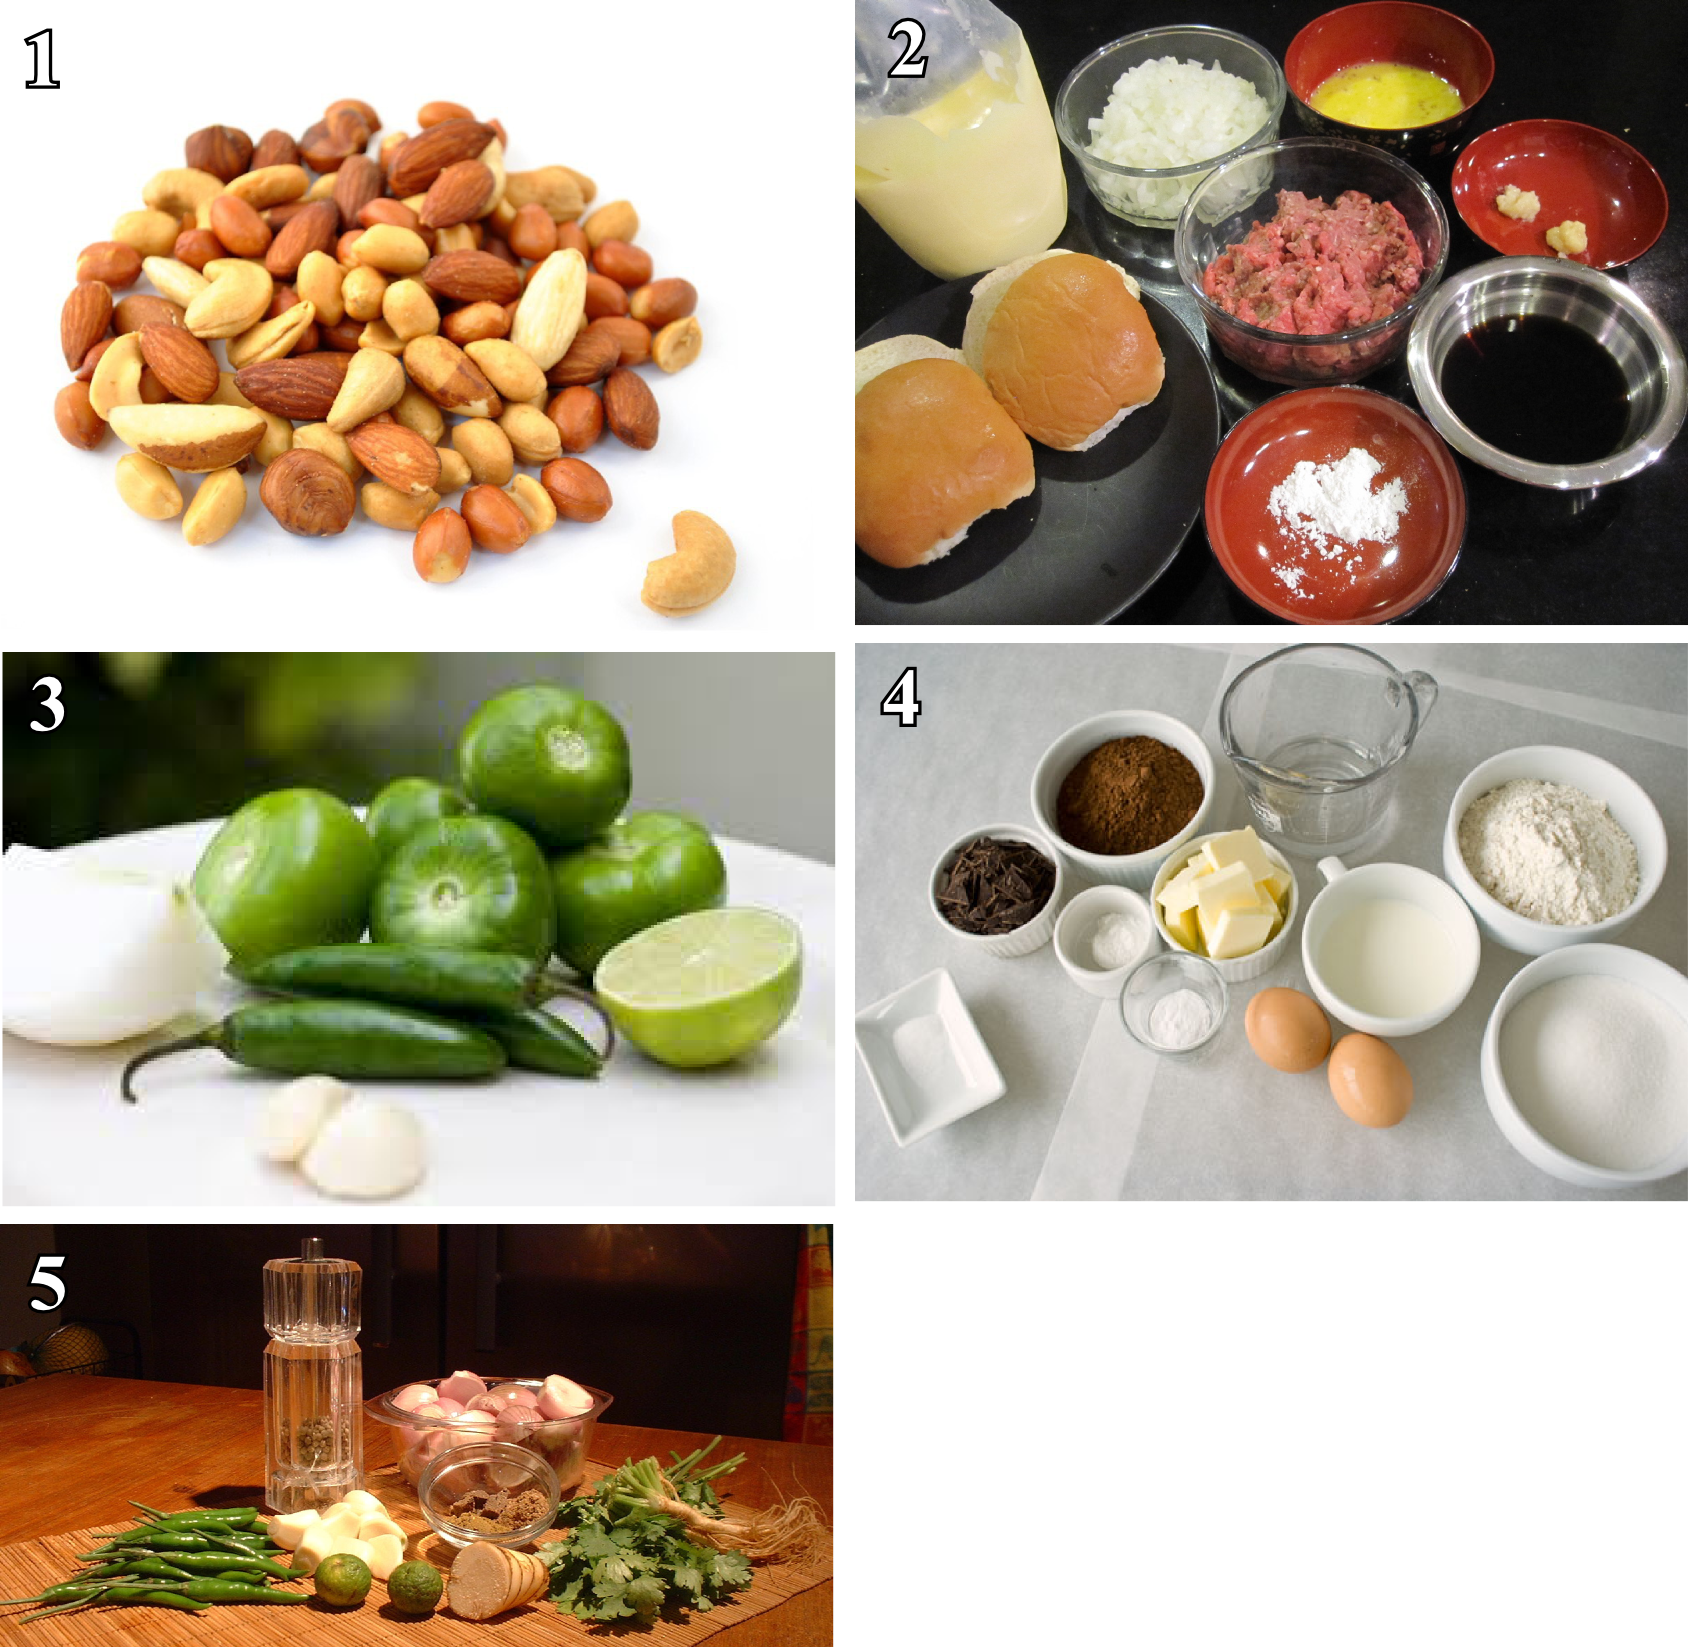
\includegraphics{figs/task2-ingr.pdf}
	\end{center}
	\caption{
		Images used in initial tasks for \textit{frame-food-culture} 
		(both for the \textit{food} and \textit{culture} treatments).
		The numbers show the order in which the images were presented to 
		workers.
	}
	\label{fig:frame2:ingr}
\end{figure}

\paragraph{Framing.}
We framed tasks by including a message, near the beginning of the HIT, that 
suggested a particular purpose for the tasks.
The precise language used is shown in 
Table~S\ref{table:experiments}, and an example of a framing slide is shown in
Fig.~S\ref{fig:hit_preamble}B and C.  In \textit{frame-food-objects}
and \textit{frame-food-culture}, the framing language was based on
naming the (fictitious) entity running the study, for example
``The Global Foundation for the Recognition of Cultures'',
or ``Laboratory for the visual perception of Objects and Tools''.
In \textit{echo-food-objects}, we stated the purpose explicitly 
(``The purpose of this task is \dots''), and then required the worker to
echo back the purpose of the task by selecting it from a combo box
Fig.~S\ref{fig:hit_preamble}C.

In \textit{frame-food-objects} and \textit{echo-food-objects}, we did not
include any initial tasks, meaning that the test tasks followed the framing
slide immediately.  One could argue that a fairer comparison would be achieved
by including initial tasks even for framing experiments (but keeping the
initial tasks constant while varying the framing language), since the worker
would be ``warmed up'' before performing the test tasks, as is the case for
the experiments investigating the effect of initial tasks. 
We therefore adopted this approach in the experiment 
\textit{frame-food-culture}, in which workers performed the same 
initial tasks containing images that depicted food in both the \textit{food}
and \textit{culture} treatments.  It would seem that the framing effect in 
\textit{frame-food-culture} was reduced by the initial tasks, possibly because
intertask effects tend to override framing. Further experimentation 
would be necessary to be sure, but this was not the purpose of our study.

\subsection*{Testing for intertask and framing effects using $\chi^2$}

\begin{table}
\centering
\begin{tabular}{c c c c}
\toprule
Experiment & Degrees of freedom & $\chi^2$ & $p$-value\\
\toprule
\textit{intertask-food-objects} & 117 & 268.7 & $6.0 \times 10^{-14}$\\
\textit{frame-food-objects} & 116 & 167.8 & $1.2 \times 10^{-3}$\\
\textit{echo-food-objects} & 126 & 381.3 & $1.7 \times 10^{-27}$\\
\textit{intertask-food-culture} & 120 & 447.5 & $2.8 \times 10^{-39}$\\
\textit{frame-food-culture} & 119 & 127.2 & $0.29$\\
\bottomrule
\end{tabular}
\caption{
	Results for Pearson's $\chi^2$ test of homogeneity of the word-frequencies
	between treatments from each experiment.  This shows that the treatments
	significantly affected word usage, 
	except in the case of \textit{frame-food-culture}.
}
\label{table:chi2}
\end{table}

\begin{table}
\centering
\begin{tabular}{c c c c c}
\toprule
Experiment & Treatment & Degrees of freedom & $\chi^2$ & $p$-value\\
\toprule
\noalign{\smallskip}
\multirow{2}{*}{\textit{intertask-food-objects}} & \textit{food} & 65 & 39.0 & $1.0$\\
 & \textit{objects} & 65 & 53.2 & $0.85$\\

\noalign{\smallskip}
\hdashline
\noalign{\smallskip}

\multirow{2}{*}{\textit{frame-food-objects}} & \textit{food} & 67 & 41.3 & $0.99$\\
 & \textit{objects} & 62 & 66.9 & $0.31$\\

\noalign{\smallskip}
\hdashline
\noalign{\smallskip}

\multirow{2}{*}{\textit{echo-food-objects}} & \textit{food} & 66 & 40.9 & $0.99$\\
 & \textit{objects} & 66 & 35.6 & $1.0$\\

\noalign{\smallskip}
\hdashline
\noalign{\smallskip}

\multirow{2}{*}{\textit{intertask-food-culture}} & \textit{food} & 62 & 65.9 & $0.34$\\
 & \textit{culture} & 68 & 57.2 & $0.82$\\

\noalign{\smallskip}
\hdashline
\noalign{\smallskip}

\multirow{2}{*}{\textit{frame-food-culture}} & \textit{food} & 57 & 49.6 & $0.75$\\
 & \textit{culture} & 64 & 55.1 & $0.78$\\

\bottomrule
\end{tabular}
\caption{
	Results for Pearson's $\chi^2$ test of homogeneity of the word-frequencies
	within treatments, which were randomly partitioned for the test.  This
	shows that word-usage within treatments is homogeneous.
}
\label{table:chi2_within}
\end{table}

To test whether intertask and framing effects induced statistically 
significant changes in word frequencies, we assembled a contingency table
for each experiment, containing the frequencies of words in each treatment.  
Any words appearing less than ten times for
an experiment (i.e. one whose expected frequency would be less than five in a 
given cell of the contingency table)
were lumped together into a separate `OTHER' category, to ensure validity
of the test.  The degrees of freedom, test statistic, and $p$-values were
then calculated according to Pearson's $\chi^2$ test, using 
Yates' correction.  Results are tabulated in Table~S\ref{table:chi2}.
With the exception of \textit{frame-food-culture}, all experiments showed 
significant changes in word-frequencies in response
to the task or framing exposures, at $\alpha=0.05$, leading us to 
reject the null hypothesis that the priming exposures had no effect.

The use of Pearson's $\chi^2$ test has been criticized in linguistic 
applications, due to the finding that many corpora are not themselves
homogeneous \cite{kilgarriff1996comparing}.  
This results from the fact that corpora are made of many
distinct texts, together with the fact that words tend to come in bursts.
When a rare word is encountered in a given text, it is much more likely
to be encountered again in the same text. This means that
frequencies within given texts are often far from the average, causing 
corpora to be heterogeneous.
As a result, if a corpus is randomly split, putting half of the texts in one 
set, and half in another, there can be a significant non-homogeneity between 
the halves (when tested using Pearson's $\chi^2$ test).  Thus, finding two
corpora to be different according to a $\chi^2$ test might not 
indicate that they are meaningfully different.

This concern does not apply to our case, because the ``texts'' are 
individual responses from workers, which will not, in general, be subject to 
the ``burstiness'' phenomenon.  Nevertheless, to test this, we randomly 
divided the workers from each experimental treatment into two sets, and 
tested the homogeneity 
between these sets.  Results are tabulated in Table~S\ref{table:chi2_within}, 
and show that treatments 
\textit{are} homogeneous.  Thus, the lack of homogeneity \textit{between} 
the treatments of given experiments can be rightly attributed to the 
framing and intertask effects.

\subsection*{Measuring the extent of intertask and framing effects}

\paragraph{Comparing $\theta$ and $\chi^2$.}
The following is an illustrative example to show why it is important to 
have a measure of effect size, like $\theta$, in addition to a test of the 
null hypothesis like $\chi^2$.
Suppose that we have a very slightly unfairly weighted coin, which turns
up heads ($X=\mathbf{H}$) more often than expected by one part in one hundred:
$\Pr\{X=\mathbf{H}\} = 0.501$. Such a coin is only mildly biased, and would 
be fine for many purposes.  If we did not know that the coin was
biased, we could determine whether it was biased by flipping the coin in 
question, along with a coin we know to be fair, many times 
(say 100 million times), and then use a $\chi^2$ test to decide whether 
the two coins have the same probability of turning up heads.
Simulating this with a random number generator yields the results shown
in Table~S\ref{table:coin}.  Results from a $\chi^2$ test of the
hypothesis that the two coins have the same probability of turning up heads 
is shown in Table~S\ref{table:coin_stats}.

\setlength{\floatsep}{30pt plus 1.0pt minus 2.0pt}

\begin{table}
\centering
\begin{tabular}{c c c c}
\toprule
coin & $N_\mathbf{H}$ & $N_{\mathbf{T}}$ & total \\
\toprule
\textit{fair} & 50002283 & 49997717 & $10^8$\\
\textit{biased} & 50101115 & 49898885 & $10^8$ \\
\bottomrule
total & 100103398 & 99896602 & $2\times 10^8$ \\
\bottomrule
\end{tabular}
\caption{
	Simulated counts of heads ($N_\mathbf{H}$) and tails ($N_\mathbf{T}$)
	occurrences, for a fair coin, and a coin biased to have a probability
	of turning up heads of 0.501.
}
\label{table:coin}
\end{table}


\begin{table}
\centering
	\begin{tabular}{c c c c }
	\toprule
	Degrees of freedom & $\chi^2$ & $p$-value \\
	\toprule
	1 & 195.4 & $2.2 \times 10^{-44}$ \\
	\bottomrule
	\end{tabular}
\caption{
	Statistics for a $\chi^2$ test of the hypothesis that a fair and 
	unfair coin have the same probability of turning up heads.  
	The result overwhelmingly favors rejection of the hypothesis, even
	though the coins differ only slightly.
}
\label{table:coin_stats}
\end{table}

Even though the $\chi^2$ test shows, with tremendous statistical 
significance, that the unfair coin is indeed unfair, we know that actual 
extent of bias is small, 
$\theta = \frac{1}{2}\left( |0.501 - 0.499| + |0.499 - 0.501| \right) = 0.002$.
This demonstrates how a sufficiently large sample size will lead to the 
detection an arbitrarily 
small bias with arbitrarily high statistical significance. 
This is why, to measure the practical significance of intertask effects,
we rely on a measure of effect size, which is in this case a measure
of statistical divergence, $\theta$.

\paragraph{Statistical approaches to measuring bias.}
Recall that Eq.~\ref{eq:theta} in the main text defined the
extent of bias between the microtask responses from two groups
of workers to be $\theta$ (reproduced here):
\begin{equation}
	\theta = \frac{1}{2}\sum_{x \in X} \left| p_0(x) - p_1(x) \right|,
\end{equation}
where $p_0(x)$ and $p_1(x)$ represent the probability that a worker from
treatment 1 (respectively 2) produces response $x$, from a set of possible
responses $X$.  As defined, $\theta$ corresponds to a measure of divergence 
between $p_0$ and $p_1$, called the \textit{total variation distance} or the
\textit{L1-distance}.

Measuring the \textit{L1-distance} between two probability distributions,
given only samples, is difficult.  The na\"ive approach is to take
the maximum likelihood estimate of $p(x)$, which sets it equal to the 
frequency with which the response $x$ has been observed, 
$\hat{p}(x) = \frac{N_x}{N}$, and then estimate $\theta$ 
using these frequencies\cite{batu2013testing}: 
$\hat{\theta} = \sum_{x \in X}|\hat{p}_1(x) - \hat{p}_2(x)|$.  
However, this method tends to drastically overestimate $\theta$
\cite{val-thesis}.
Recently there has been theoretical progress on this problem.
An estimator of L1-distance, and tests of whether the L1-distance is
greater than a specified threshold, have been proposed 
\cite{val-thesis,batu2013testing,chan2014optimal}.  
These methods have excellent theoretical convergence guarantees, but
cannot easily be used to establish estimates with confidence intervals or 
perform hypothesis tests for fixed sample size and significance level.  
We therefore turn to an alternative approach using machine learning. 
While this method yields an estimator that converges more slowly,
it is straightforward to establish confidence intervals and 
use the estimator in hypothesis tests.

\paragraph{The relationship of bias and classifier accuracy.}
We will now show that, any classifier algorithm, $\mathcal{A}$, that
takes the response, $x$, of a worker, and guesses the population to which
the worker belongs ($P_0$ or $P_1$), will do so with an accuracy, $\eta$,
that is bounded according to Eq.~\ref{l1} from the main text 
(reproduced here):
\begin{equation}
	\theta \geq 2\eta - 1.
	\label{eq:sup:l1}
\end{equation}

To do so, we will first formalize $\eta$ by defining a 
\textit{validation test}.  In a validation test, a uniform random bit 
$z\in\{0,1\}$ is sampled, and then, according to the value of $z$, the
response of a worker, $x$, is sampled uniformly randomly from $P_z$.  
The algorithm is provided
with $x$ and yields a \textit{guess}, $b=\mathcal{A}(x)$, as to whether the 
worker was 
from $P_0$ or $P_1$.  We shall denote such a validation test by 
$V(P_0, P_1, \mathcal{A})$, and define the value of the test to be 1 if 
$b=z$ and 0 otherwise.  

We then define the accuracy of classifier $\mathcal{A}$ to be $\eta$ according
to:
\begin{equation}
\eta = \mathrm{E\{V(P_0, P_1, \mathcal{A})\}} 
	= \mathrm{Pr}\{V(P_0, P_1, \mathcal{A})=1\}.
\end{equation}

To develop the relationship between $\eta$ and $\theta$, let us consider
the accuracy $\eta^*$ of the best possible classifier $\mathcal{A}^*$.
The best possible classifier will not in general have perfect accuracy:
if the responses from workers in $P_0$ and $P_1$ are distributed 
identically, then there is no hope of determining which population the worker 
came from given only her response $x$.  But, assuming that responses are
not distributed identically, then given some $x$, the best possible 
classifier must always guess 1 whenever $p_1(x) > p_0(x)$ and guess 0 whenever
$p_0(x) > p_1(x)$.

Sacrificing, for a moment, some generality, let us assume that, for some give 
$x'$, $p_1(x') > p_0(x')$.  
When this $x'$ is encounterend in a validation test, the optimal classifier
must guess $b = \arg\!\max_{z}(p_{z}(x'))$, which in this case is $b=1$.
The probability that the classifier guesses correctly in this case is:
\begin{align}
	\begin{split}
	\mathrm{Pr}\{V(P_0, P_1, \mathcal{A}^*) = 1 | x = x' \} 
		&= \mathrm{Pr}\{z = \mathcal{A^*}(x) | x = x' \} \\
		&= \mathrm{Pr}\{z = 1 | x = x' \}  \\
		&= \frac{\mathrm{Pr}\{z = 1 , x = x'\}}
			{ \mathrm{Pr}\{z=0 , x=x'\} + \mathrm{Pr}\{z=1 , x=x'\}} \\
		&= \frac{p_1(x')}{p_0(x') + p_1(x')}.
	\end{split}
\end{align}
And now, with full generally, for any $x'$, where $p_1(x')$ is not necessarily
greater than $p_0(x')$:
\begin{align}
	\begin{split}
		\mathrm{Pr}\{V(P_0,P_1,\mathcal{A}^*)=1 | x = x' \} 
		&= \mathrm{Pr}\{z=\mathcal{A^*}(x)  | x' = x' \} \\
		&= \mathrm{Pr}\{z = \arg\!\max_{z'}\big(p_{z'}(x)\big)| x = x' \}  \\
		&= \frac{\max\big( p_0(x'),p_1(x') \big)}
		{ p_0(x') + p_1(x') }.
	\end{split}
\end{align}
Note that we can rewrite $\max\big(p_0(x'),p_1(x')\big)$:
\begin{align}
	\max\big(p_0(x'),p_1(x')\big) = \frac{1}{2}
		\big(
			p_0(x') + p_1(x') + |p_0(x') - p_1(x')|
		\big),
\end{align}
so,
\begin{align}
	\mathrm{Pr}\{V(P_0,P_1,\mathcal{A}^*) = 1 | x = x' \} 
	&= \frac{1}{2} + \frac{|p_0(x') - p_1(x')|}{2 \big(p_0(x') + p_1(x') \big)}.
\end{align}
Then, summing over all possible responses $X$, 
the overall accuracy of the optimal classifier, $\mathcal{A^*}$, is:
\begin{align}
	\begin{split}
	\eta^* &= \mathrm{Pr}\{V(P_0, P_1, \mathcal{A}^*)=1\} \\
	&=\sum_{x'\in X} \mathrm{Pr}\{V(P_0,P_1,\mathcal{A}^*) = 1 | x = x' \} \mathrm{Pr}\{x = x'\}\\
		&= \sum_{x'\in X} \left(
				\frac{1}{2} + 
				\frac{|p_0(x') - p_1(x')|}{2 \big(p_0(x') + p_1(x') \big)}
			\right)
			\left(
				\frac{p_0(x') + p_1(x')}{2}
			\right)\\
		&= \frac{1}{2}\left(
				\frac{1}{2}(
					\sum_{x' \in X}p_0(x') + \sum_{x' \in X}p_1(x')
				) + 
				\frac{1}{2} \sum_{x' \in X} \big(|p_0(x') + p_1(x')|\big)
			\right) \\
		&= \frac{1}{2} \left( \frac{1}{2}(1 + 1) + \theta \right)\\
		&= \frac{1 + \theta}{2}\\
		\implies \theta &= 2\eta^* - 1.
	\end{split}
\end{align}
By definition, no classifier can be more accurate than $\mathcal{A^*}$, so
for every $\mathcal{A}$
\begin{align}
		\theta \geq 2\eta - 1.
		\label{eq:sup:l1_again}
\end{align}

\paragraph{Using cross-validation accuracy to lower-bound bias.}
	In order for Eq.~\ref{eq:sup:l1_again} to be applicable, it is necessary to 
	obtain an unbiased estimate of a classifier's accuracy.  To do so, it is
	essential to test the classifier on data that were not used to build 
	the classifier.  Generally, a portion of the data is used to
	optimize preprocessing, select features, and optimize 
	classifier hyper-parameters, while keeping another portion of the data
	set aside for validation.

	In our case, the data are expensive, and must be divided between 18
	experimental treatments, so we sought to keep as many worker responses
	available 
	for validation
	as possible.  For this reason, we made principled decisions 
	between alternative preprocessing options and features, 
	rather than spending sampled responses on empirically testing these 
	options.  Making
	suboptimal choices can only moderate the observed values 
	of $\theta$, making our experiments more conservative. 
	However, conserving more responses for validation 
	tests, by not using them for classifier optimization, 
	enables us to estimate the resulting classifier's accuracy more precisely.
	Using a Na\"ive Bayes classifier, which does not require hyper-parameter 
	optimization, meant that we also did not need to spend data on 
	optimizing hyper-parameters.  
	
	Thus, no worker responses at all were used for optimizations.  We 
	performed 
	leave-one-out validation, which involves training a classifier using 
	all but one response, and then having the classifier guess the class
	(in our case, the priming exposure) of the left-out worker.  This is 
	repeated $n$ times, where $n$ is the pooled number of worker responses 
	in both
	classes (both treatments in a given experiment), 
	each time leaving out the response of a different worker.

\paragraph{Selection of the na\"ive Bayes classifier.}
We chose to use the na\"ive Bayes classifier as our basis for measuring 
bias for three reasons.  First, we had 119 examples (workers) per class 
(treatment), but thousands of distinct features 
(i.e. the number of distinct words occurring in an experiment).  
Having many more features than examples is problematic for many classifiers
because a large number of features leads to a high-variance, over-fit model,
resulting in poor performance.  But one of the strengths of the na\"ive 
Bayes classifier is that it performs well even when the number of features
exceeds the number of examples\cite{bickel2004, hastie2009elements}

Second, the standard implementation of the na\"ive Bayes classifier has no 
hyper-parameter to optimize. This meant that we did not need to use 
samples for hyper-parameters optimization, which would reduce the number
of samples available for validation tests to estimate $\theta$.

Third, the na\"ive Bayes algorithm is based on an assumption that the 
observation of one feature is independent from the observation of any 
other, once we have conditioned on the class under observation 
\cite{bishop2006} (i.e. the priming treatment).  This
conditional independence assumption is made for
pragmatic rather than theoretical reasons, and is rarely satisfied.  However,
if it \textit{is} satisfied, then the na\"ive Bayes classifier is 
optimal \cite{Zhang2004562}.  In most text documents, 
the existence of long-range dependencies in language 
violates the conditional independence of words: when a rare word is mentioned,
it is more likely to be mentioned again, and topics introduced early in a
text are likely to be revisited.
But in our case, there is little opportunity for such effects.  Workers 
generally do not use the same word in multiple labels for the same image. 
Any overarching ``topics'' within the labels that workers use will tend to 
relate to the test images, which are held in common.
Therefore, in our setup, conditional independence is likely to be 
a realistic approximation, and so the na\"ive Bayes classifier is likely to
be closer to optimal than in other text classification applications.

\paragraph{Comparison to other classifiers.} 

\begin{figure}
	\centering
	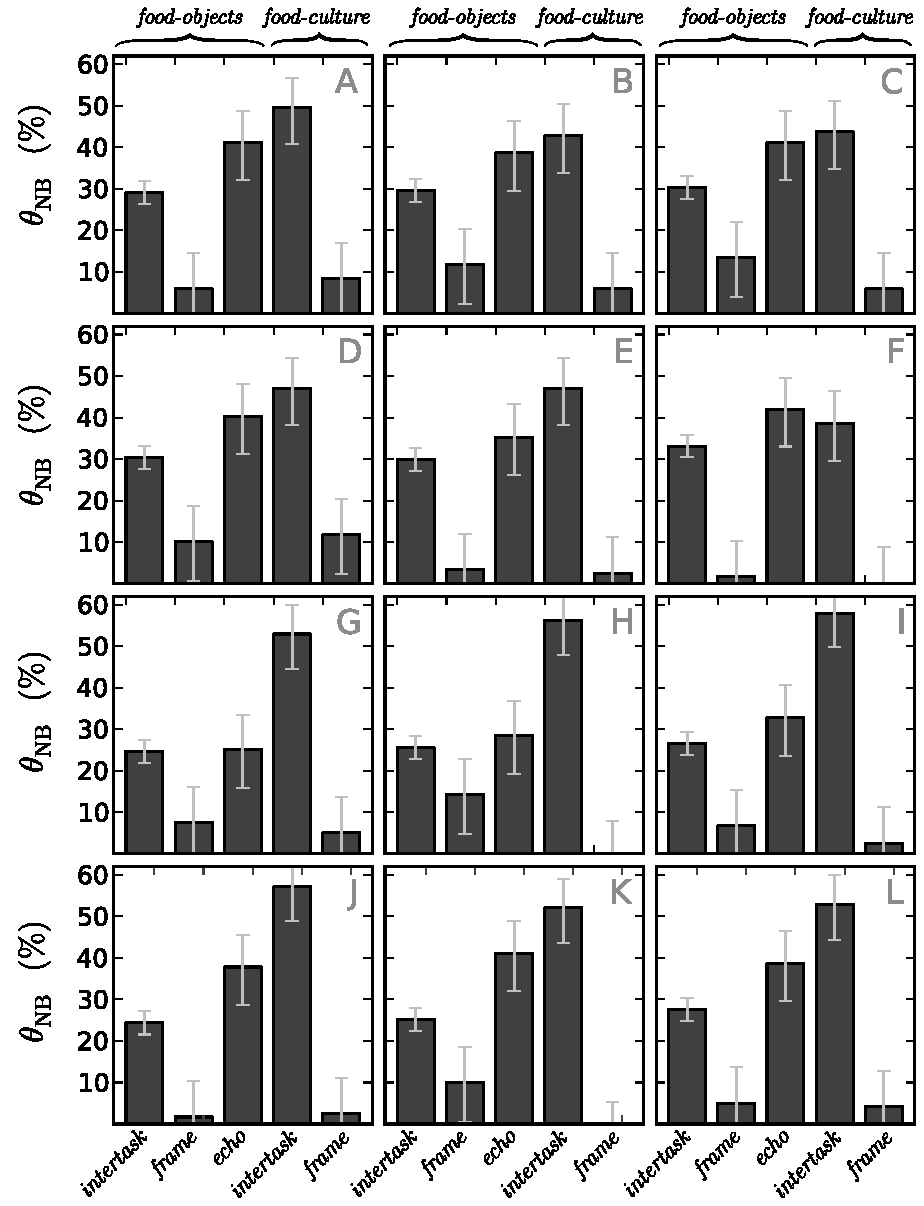
\includegraphics[scale=0.75]{figs/theta_sup.pdf}
	\caption{
		Empirical bias, measured using classifiers, induced in image 
		labeling tasks, by exposing workers to initial tasks or framing. 
		The bias was determined using (A-F) a na\"ive Bayes classifier, and 
		(G-L) an SVM classifier, according to Eq.~\ref{eq:sup:l1}.
		In panels A through F, each plot adds an additional
		preprocessing step to those used in the previous plot; the same is 
		done for panels G through H: A,G) no 
		preprocessing; B,H) spelling correction; C,I) stop word removal; 
		D,J) lemmatization; E,K) splitting of multiple-word labels; 
		F,L) distinguishing identical labels entered in different form inputs.
		Standard error bars are shown.
	}
	\label{fig:theta_sup}
\end{figure}
The inequality in Eq.~\ref{eq:sup:l1_again}
asserts that a classifier's performance in predicting class membership
sets a lower bound on the L1-distance between the distributions of features 
for the classes.
This bound is tight for the optimal classifier, and in general, the slack
depends on how the classifier is constructed.

Although we believe the na\"ive Bayes classifier is nearly optimal in this
setting, some other classifier may exist that is significantly better than 
the one used to generate our results.  Furthermore, various decisions about
preprocessing and feature representation also
impact the classifier performance.  
For example, we chose to correct spelling, remove stop words,
lemmatize words, and to distinguish which text-input was used to enter a 
given label.  All of these decisions have some effect on classifier 
performance.

We chose not to optimize these decisions, since it would require the
use of samples (worker-responses), which could then not be used in 
cross-validation to measure $\theta$.  Nevertheless, it is
appropriate to look at what affect these decisions had, \textit{post-hoc}.  
We reproduce the plot from Fig.~\ref{fig:theta}A in the main text, 
this time using different combinations of preprocessing options,
and using both the na\"ive Bayes and an SVM classifier, in 
Fig.~S\ref{fig:theta_sup}.

Unlike the na\"ive Bayes classifier, when using SVM it is necessary to tune 
the cost and gamma hyper-parameters of the SVM classifier, as well as choose 
a kernel.  We used simulated annealing to optimize the cost and gamma settings
data from \textit{intertask-food-culture}.  For this reason, the estimate
of $\theta$ estimate for this experiment in 
Fig.~S\ref{fig:theta_sup} (G to J) is inflated. 

These plots suggest that the values of $\theta$ obtained using the 
na\"ive Bayes classifier and our particular choice of preprocessing steps, 
as shown in in Fig.~\ref{fig:theta} of the main text, are representative.

\paragraph{Statistical significance and confidence intervals for $\theta$.}
The measurements of $\theta$ were based on the number of correct 
classifications during validation tests.  The number of correct 
classifications, $X$, has a binomial distribution.  
We take the null hypothesis that the classifier performs
no better than chance, $X \sim \mathrm{Bin}(N,0.5)$, where $N$ is the number 
of workers in both treatments of an experiment, and consider an alternative
hypothesis, that the classifier does perform better than chance.  Then, the 
critical number 
of correct classifications, $x^*$, for a one-tailed hypothesis test with
significance $\alpha$ is:
\begin{align}
	&x^* = \sup \left\{
			x: \mathrm{Pr}\{ \mathrm{Bin}(N;0.5) \geq x \} < \alpha
		\right\} \label{eq:sup:crit}\\
	\text{where}\quad &\mathrm{Pr}\{ \mathrm{Bin}(N,\eta) \geq x \} = 
		\sum_{x'=x}^{N} \binom{N}{x'}\eta^{x'}(1-\eta)^{(N-x')}
\end{align}
For the treatments in \textit{intertask-food-objects}, five different 
permutations of each treatment were tested, and a different classifier was 
built for each permutation.  For the sake of estimating accuracy, we assume
that the classifiers under different permutations have the same accuracy,
and so we pool their results.  This means that 
\textit{intertask-food-objects} has five times as many validation tests
(larger $N$) compared to the other experiments.  This larger $N$ makes 
evaluation of \ref{eq:sup:crit} difficult, but also makes the normal 
distribution a very good approximation.  We therefore assume 
that $X$ has a normal distribution for the classification of workers from
\textit{intertask-food-objects}, with $\mu=N/2$ and 
$\sigma = \frac{1}{2}\sqrt{N}$.  The statistics for these hypothesis tests
are tabulated in Tables~S\ref{table:theta} and S\ref{table:theta_pos}.

To determine the confidence intervals for measured $\theta$ values we 
use the exact Clopper-Pearson method \cite{clopper1934use}.  
Based on the observed number of successes, $X$, we calculate 
$\eta^*_\mathrm{low}$ and $\eta^*_\mathrm{high}$ from:
\begin{align}
	\eta^*_\mathrm{high} &= \sup
		\left\{
			\eta : \mathrm{Pr}\{\mathrm{Bin}(N; \eta) \leq X \} > 
				\frac{\alpha}{2}
		\right\} \\
	\eta^*_\mathrm{low} &= \inf
		\left\{
			\eta : \mathrm{Pr}\{\mathrm{Bin}(N; \eta) \geq X \} > 
				\frac{\alpha}{2}
		\right\}
\end{align}
Again, for the experiment \textit{intertask-food-objects}, which had 
more validation tests than the others, we derive the confidence intervals
assuming $X$ is normally distributed.
Since the confidence intervals are to be shown on a plot of $\theta$, we 
transform them into equivalent values of 
$\theta$: $\theta^*_\mathrm{high} = 2\eta^*_\mathrm{high} - 1$ and 
$\theta^*_\mathrm{low} = 2\eta^*_\mathrm{low} - 1$.
The statistics collected for the measurement of $\theta$, corresponding to
Figs.~\ref{fig:theta}A and B are tabulated in Tables~S\ref{table:theta} and
S\ref{table:theta_pos} respectively.

To determine whether intertask effects were stronger than framing, we 
perform a two-proportion $z$-test, approximating the binomial distributions
as normal distributions, where the test statistic is given by:
\begin{align}
	z = \frac{\hat{\eta}_1 - \hat{\eta}_2}
		{\sqrt{
			\hat{\eta} (1 - \hat{\eta}) 
			\left( \frac{1}{N_1} + \frac{1}{N_2}\right)
		}},
\end{align}
where
\begin{align}
	\hat{\eta} = \frac{X_1 + X_2}{N_1 + N_2}
\end{align}


Since, \textit{a priori}, we do not know which effects
should be stronger (if any), we perform a two-tailed test.  The results for 
these hypothesis tests are tabulated in Table~S\ref{table:intertask_framing}.
The results show that intertask effects are stronger than framing, but are
on-par with echoed framing.


\begin{table}
\begin{center}
\begin{tabular}{c c c c c c c c }
	\toprule
	\multirow{2}{*}{Experiment} & \multirow{2}{*}{$N$} & 
	\multirow{2}{*}{$X$} & \multirow{2}{*}{$x^*$} & \multicolumn{3}{c}{(\%)}
		& \multirow{2}{*}{$p$}\\ \cline{5-7} \noalign{\smallskip}
	& & & & $\hat{\theta}$ & $\theta^*_\mathrm{low}$ 
		& $\theta^*_\mathrm{high}$  \\
	\midrule
	\textit{intertask-food-objects} & 1190 & 777 & 624 & \textbf{30.6} 
		& 25.2 & 36.0 & $2.5 \times 10^{-26}$ \\
	\textit{frame-food-objects} & 238 & 122 & 133 & 2.5 & -10.6 & 14.7
		& 0.37 \\
	\textit{echo-food-objects} & 238 & 162 &  133 & \textbf{36.1} & 23.4 
		& 47.1 & $1.3 \times 10^{-8}$ \\
	\textit{intertask-food-culture} & 238 & 180 & 133 & \textbf{51.3} & 39.3 
		& 61.1 & $5.0 \times 10^{-16}$ \\
	\textit{frame-food-culture} & 238 & 130 & 133 & 9.2 & -3.9 & 21.3 
		& 0.087\\
	\bottomrule

\end{tabular}

\caption{Statistics for the measurement of the extent of bias, $\theta$,
	induced by intertask and framing effects in various experiments.
	Number of validation tests, $N$; number of successful classifications, 
	$X$; critical number of successful classifications to reject the null 
	hypotheses that the classifier does no better than chance 
	(one-tailed test), $x^*$; 
	estimate of bias based on observed number of successful
	classifications, $\hat{\theta}$; lower confidence interval limit 
	for the estimate of bias, $\theta^*_\mathrm{low}$; upper confidence 
	interval limit for same, $\theta^*_\mathrm{high}$.  Hypothesis test and 
	confidence intervals are based on a significance of $\alpha=0.05$.
	Values for $\hat{\theta}$ in boldface are significantly greater than zero.
}
\label{table:theta}
\end{center}
\end{table}

\begin{table}
\begin{center}
\begin{tabular}{c c c c c c c c }
	\toprule
	\multirow{2}{*}{Task position} & \multirow{2}{*}{$N$} & 
	\multirow{2}{*}{$X$} & \multirow{2}{*}{$x^*$} & \multicolumn{3}{c}{(\%)}
		& \multirow{2}{*}{$p$}\\ \cline{5-7}\noalign{\smallskip}
	& & & & $\hat{\theta}$ & $\theta^*_\mathrm{low}$ 
		& $\theta^*_\mathrm{high}$  \\
	\midrule
	1 & 238 & 152 & 133 & \textbf{28.1} & 14.8 & 39.1 
		& $1.12 \times 10^{-5}$\\
	2 & 238 & 138 & 133 & \textbf{15.6} & 2.9 & 27.8  
		& $8.14 \times 10^{-3}$\\
	3 & 238 & 140 & 133 & \textbf{17.8} & 4.6 & 29.5  
		& $3.87 \times 10^{-3}$\\
	4 & 238 & 135 & 133 & \textbf{13.6} & 0.3 & 25.4  
		& $0.0221$ \\
	5 & 238 & 134 & 133 & \textbf{12.4} & 0.5 & 24.6 & $0.0300$ \\
	\bottomrule
\end{tabular}
\caption{Statistics for the measurement of the extent of bias, $\theta$,
	induced by intertask for \textit{intertask-food-objects}, measured 
	for test images at specific positions in the sequence of five test images.
	These values are averaged over five different permutations.
	Number of validation tests, $N$; number of successful classifications, 
	$X$; critical number of successful classifications to reject the null 
	hypotheses that the classifier does no better than chance 
	(one-tailed test), $x^*$; 
	estimate of bias based on observed number of successful
	classifications, $\hat{\theta}$; lower confidence interval limit
	for the estimate of bias, $\theta^*_\mathrm{low}$; upper confidence 
	interval for same, $\theta^*_\mathrm{high}$.  Hypothesis test and 
	confidence intervals are based on a significance of $\alpha=0.05$.
	Values for $\hat{\theta}$ in boldface are significantly greater than zero.
}
\label{table:theta_pos}
\end{center}
\end{table}



\begin{table}
\begin{center}
\begin{tabular}{c c c c c c c c c c c }
	\toprule
	Comparison & $N_1$ & $N_2$ & $X_1$ & $X_2$ & $\hat{\eta}_1$ 
		& $\hat{\eta}_2$ & $z$ & $p$-value \\ 
	\midrule
	\parbox[c]{4cm}{\textit{intertask-food-objects} 
	\textit{vs} \textit{frame-food-objects}} & 1190 & 238 & 777 & 122 &
	0.653 & 0.513 & \textbf{4.1} & $2.1 \times 10^{-5}$ \\ 

\noalign{\smallskip}
\hdashline
\noalign{\smallskip}

	\parbox[c]{4cm}{\textit{intertask-food-objects} 
	\textit{vs} \textit{echo-food-objects}} & 1190 & 238 & 777 & 162 
		& 0.653 & 0.681 & -0.82 & 0.79 \\

\noalign{\smallskip}
\hdashline
\noalign{\smallskip}

	\parbox[c]{4cm}{\textit{intertask-food-culture} 
	\textit{vs} \textit{frame-food-culture}} & 238 & 238 & 180 & 130 
	& 0.756 & 0.546 & \textbf{4.8} & $7.6 \times 10^{-7}$ \\
	\bottomrule

\end{tabular}

\caption{
	Results for two-proportion z-tests, testing the null hypothesis that 
	intertask and framing effects are equally strong.
	In the cases of comparing intertask effects to passive framing, the
	null hypothesis should be rejected ($\alpha=0.05$), but 
	echoed framing effects are on par with intertask effects (second row). 
	$z$-statistics in boldface are significantly different from zero.
}
\label{table:intertask_framing}
\end{center}
\end{table}




\subsection*{Data preprocessing}
	\paragraph{Splitting, lemmatization, removal of stop words, and 
		addition of position tags.} 

	Before performing any analysis on the labels that workers provided, we
	performed a series of preprocessing steps.  
	Labels that contained
	multiple words (separated by spaces or punctuation) were split, with
	punctuation removed, and the separated words were treated as distinct 
	features in subsequent analysis.
	Misspelled words were automatically corrected using a spelling 
	correction algorithm described below.  
	Next, words were lemmatized using the
	wordnet lemmatizer \cite{miller1995wordnet,felbaum1998wordnet}.  
	Common words such as ``the'', ``to'', or ``with'', were found using
	NLTK's English stop word list \cite{loper2002nltk} and removed.

	For the purpose of training and testing a na\"ive Bayes classifier, we 
	performed an additional preprocessing step.  We tagged words with the
	position in which they had been entered (i.e. which of the five text 
	inputs in the task interface, Fig.~S\ref{fig:hit_preamble}) 
	as well as the test tasks in which the word had been provided.
	So, if the word ``wine'' was entered into the second text-input for 
	the third test-task, after preprocessing, the feature ``3\_2\_wine'' would
	appear.  Prepending the task number onto words was simply a means to 
	retain correct attribution of words to images, since providing a word 
	during one task 
	is not equivalent to providing the same word during another task.  
	
	\paragraph{Spelling correction.}  
	Spelling correction was performed using an algorithm that first detected
	if a word was likely to be misspelled, then generated a set of candidate 
	corrections, and chose the best candidate based on a scoring mechanism.
	
	A word was considered misspelled if it was not contained in the 
	\textit{legal set}, which was formed by the union of
	the wordnet corpus, the stop word list, and a set of words seen while 
	crawling the world food section of the allrecipes.com website.  We
	describe the crawling of the allrecipes.com website in a section below.

	To correct misspellings, we first produced all possible modified forms 
	that could be obtained applying one or two edits.  An edit consisted of 
	adding or removing a letter, changing one letter into another, or 
	swapping the positions of two adjacent letters.  For the purpose of these 
	edits, spaces were treated as any other letter.

	The candidates produced by these edits which were in the legal set were
	then ranked based on a scoring mechanism, and the highest scoring word
	was chosen as the correction.  A candidate $w$'s score, $s_w$, was 
	calculated according to the following formula:
	\begin{equation}
		s_w = (f_w + 1) \times p_1 \times p_2,
	\end{equation}
	where $f_w$ is the frequency with which the word occurred (correctly 
	spelled)
	within the given task, $p_1$ was a penalty for the first edit, and
	$p_2$ was a penalty for the second edit.  If the word was made using only
	one edit, then $p_2 = 1$.  Any edit that did not involve adding a space
	(i.e. separating a word) incurred a penalty of 0.5, while the addition of
	a space incurred a penalty of 0.1.  Word-separation edits were more 
	strongly penalized because it is often possible to split a series of 
	letters into short two- or three-letter words, which leads 
	to many erroneous corrections.  We found these penalties worked well when
	testing on words taken from initial tasks.

	After all of our analyses had been performed, we checked the accuracy of 
	the spelling correction algorithm using three human coders.  The coders
	were shown a set of 
	500 words that were randomly sampled from the labels attributed during 
	test tasks (50 for each test task).  Before sampling, the labels from all
	experimental treatments, for the given test task, were pooled together.
	The coders did not know which treatment any given word came from.  
	In addition to the words, coders were shown the spelling correction 
	produced by the algorithm, as well as the image from the test task.
	The coders were asked to identify any misspelled words which had not 
	been corrected, as well as any corrections that appeared to be erroneous,
	by indicating their own correction.

	According to the human coders, before spelling correction, 17\% of words 
	were misspelled, but only 3.2\% were misspelled after correction.

	\paragraph{Crawling the world food section of allrecipes.com.}
	The website allrecipes.com was accessed on 3-4 November 2014 using 
	automated scripts.  A total of 2642 recipe listings and 15621 recipe
	instruction pages were retrieved.  Recipe listings were pages that 
	provided lists of recipes, and contained a title and short description 
	for each.  
	The recipe instruction pages had lists of ingredients and preparation 
	instructions.  All of the words found in recipe titles, short
	descriptions, ingredients lists, and preparation instructions were
	collected, and saved as an auxiliary set to augment the \textit{legal set}
	used in spelling correction.
	

\subsection*{Analysis of worker vocabulary}
\paragraph{Most suppressed and activated terms.}
The words whose frequencies differed most between the treatments of given 
experiments are shown in Table~S\ref{table:top-words}.  Note that 
the word that was most suppressed in food-exposed treatments was always 
``food''.

\begin{table}
	\centering
	\setlength{\tabcolsep}{4pt}
	\begin{tabular}{ c c c c c }
	
		\setlength{\tabcolsep}{4pt}
		\begin{tabular}{ r | c }
		\toprule
		\multicolumn{2}{c}{
			\parbox[c]{2.5cm}{
				\centering
					\textit{intertask-food-objects}
			}} \\
		\midrule
		coffee & 38 \\
		meal & 34 \\
		cheese & 34 \\
		apple & 32 \\
		dessert & 21 \\
		cup & -30 \\
		glass & -45 \\
		table & -70 \\
		candle & -74 \\
		food & -80 \\
		\bottomrule
		\end{tabular}

&

		\setlength{\tabcolsep}{4pt}
		\begin{tabular}{ r | c }
		\toprule
		\multicolumn{2}{c}{
			\parbox[c]{2.5cm}{
				\centering
				\textit{frame-food-objects}
			}
		}\\
		\midrule
		bread & 18 \\
		wine & 18 \\
		cheese & 16 \\
		apple & 14 \\
		oil & 12 \\
		table & -9 \\
		meal & -10 \\
		candle & -12 \\
		dinner & -13 \\
		food & -32 \\
		\bottomrule
		\end{tabular}

&

		\setlength{\tabcolsep}{4pt}
		\begin{tabular}{ r | c }
		\toprule
		\multicolumn{2}{c}{
			\parbox[c]{2.5cm}{
				\centering
			\textit{echo-food-objects}} 
		}\\
		\midrule
		apple & 24 \\
		cheese & 23 \\
		wine & 15 \\
		coffee & 14 \\
		oil & 7 \\
		knife & -24 \\
		dinner & -26 \\
		fork & -27 \\
		candle & -35 \\
		food & -55 \\
		\bottomrule
		\end{tabular}

&

		\setlength{\tabcolsep}{4pt}
		\begin{tabular}{ r | c }
		\toprule
		\multicolumn{2}{c}{
			\parbox[c]{2.5cm}{
				\centering
			\textit{intertask-food-culture}} 
		}\\
		\midrule
		spicy & 26 \\
		sauce & 17 \\
		indian & 15 \\
		buffet & 14 \\
		exotic & 12 \\
		festival & -11 \\
		offering & -12 \\
		statue & -15 \\
		india & -20 \\
		food & -56 \\
		\bottomrule
		\end{tabular}

&

		\setlength{\tabcolsep}{4pt}
		\begin{tabular}{ r | c }
		\toprule
		\multicolumn{2}{c}{
			\parbox[c]{2.5cm}{
				\centering
			\textit{frame-food-culture}} 
		}\\
		\noalign{\smallskip}
		\midrule
		indian & 11 \\
		banquet & 8 \\
		spicy & 7 \\
		asian & 6 \\
		variety & 6 \\
		delicious & -6 \\
		meat & -7 \\
		festival & -7 \\
		spice & -7 \\
		food & -9 \\
		\bottomrule
		\end{tabular}

	\end{tabular}
	\caption{
		The five words whose frequencies increased, and those whose 
		frequencies decreased, the most, between treatments of given 
		experiments, within labels attributed to the first test task.
		Positive values indicate that the food-exposed treatment
		used the word with higher frequency.  
		Note that the word ``food'' is always the most suppressed among
		food-exposed workers.
		Word frequencies for 
		\textit{intertask-food-objects} correspond to the labels attributed
		to image 1 (see Fig. \ref{fig:task1:test}) which is not necessarily 
		the first 
		test task due to the tasks being permuted.  There were five times
		as many workers in \textit{intertask-food-objects}, hence
		larger absolute differences are observed.
	}
	\label{table:top-words}
\end{table}

\paragraph{Identification of food-related terms.}
The wordnet corpus is composed of synsets, which are particular senses 
(meanings) and a set of word forms bearing that meaning. A given word form, 
such as ``ring'' has multiple senses (``to ring a bell'', ``a wedding ring''),
and so can be part of many synsets.  Since the wordnet corpus was designed
to carry semantic information, the synset is the basic organizing element
of wordnet.

We chose the synsets \texttt{food.n.01} and \texttt{food.n.02} to act as roots
in defining which words should be considered food-related.  Any word form
belonging to a synset which was a hyponym of one of the two root synsets
identified above was considered to be a reference to food.  Here, as in the
main text, when we say hyponym, we mean either a direct hyponym, or a hyponym
of a hyponym, and so on.

This is a stringent notion of a word being a food reference.  It roughly
corresponds to whether or not a given thing is reasonably considered 
consumable.  So, ``orange'' is food, but ``salty'' is not.  Although ``salty''
would usually qualify something edible, it is not itself an edible thing.
On the other hand, ``salt'' would be considered a reference to food under 
this operationalization.

The subset of the wordnet corpus induced by the hyponyms of \textit{food.n.01}
and \textit{food.n.02} consists of 3590 word-forms.  Manual
testing showed good coverage, except for references to ethnic foods.  
Since, especially in \textit{intertask-food-culture} and 
\textit{frame-food-culture}, we had images containing many ethnic 
foods, we decided to augment the wordnet corpus with words learned by 
crawling the world food section of the allrecipes.com website.  

After collecting a set of words using an automated script 
(described above), we filtered down to the set of words that had been used by
workers and which had been seen during crawling of the allrecipes.com website,
but which were not included in wordnet.  We grafted these extra words into
the wordnet hyponym-hypernym graph manually, looking at the image to which 
they had been attributed (to help disambiguate the intended meaning), but 
without revealing the treatment(s) in which
the word was used.  Many (but not all) of the words added this way did refer 
to ethnic foods, and so this helped increase the coverage of wordnet in that 
respect.

\paragraph{Validation of the detection of food references.}
To determine whether our extended version of wordnet provided a good approach
to detecting food-related words, we sampled 500 words 
(50 from each test task)  from the set of labels produced by workers and had 
three human coders manually decide if they were 
food-related or not.

The coders were instructed to consider whether a word was a noun signifying
an edible item.  The guiding principle was, for the coder to ask herself,
``can I eat X'', where X is the word she is coding.  The coders were
shown the image used in the task from which the word came, to help resolve ambiguity
in the sense of the word that had been given.  Coders were also shown the 
spelling correction (if any) that the spell-correction algorithm had made,
to help interpret misspelled words.

We evaluated the food detection algorithm in two ways.  First, we measured
the inter-rater reliability between the three human coders and the algorithm
(treating the algorithm just like any other coder).  Second, adopting the 
majority code given by the human coders as ground-truth, we determined the 
accuracy of the food-detection algorithm.  
Data summarizing this validation process are given
in Table~S\ref{table:inter-rater}.

\begin{table}
\centering
\setlength{\tabcolsep}{12pt}
\begin{tabular}{ r | c }
\toprule    
\# terms coded & 500 \\
\# food references & 130 \\
\# correct machine codes & 440 \\
inter-rater reliability & 82.4\% \\
human-machine code agreement & 88\% \\
%machine recall & 80 \% \\
%machine precision & 75.4 \% \\
%machine code F1 & 0.78 \\
\bottomrule
\end{tabular}
\caption{
	Results for the validation 
	of the automatic detection of food references, by comparison to
	human-generated coding on randomly sampled words.  In calculating the 
	human-machine code agreement, the majority human code was used.
	Inter-rater reliability was calculated as Krippendorff's alpha, treating
	the machine as any other coder.
}
\label{table:inter-rater}
\end{table}

The results show that good inter-rater reliability was achieved during the
validation (82.4\%).  Looking at the agreement between the 
machine codes and the majority human-generated codes, we find they agree
88\% of the time.  This means that the concept used to instruct human coders
provides a good approximation to what the wordnet-based machine codes actually
represent. In other words, the machine codes correspond closely to indicating
which words correspond to nouns that refer to edible things, and which ones
do not, which provides a clear and simple interpretation for the machine
coding of food and non-food words.

\paragraph{Testing differences in proportions of food-related labels.}
We calculate the proportion of food-related labels in a treatment by first
calculating the proportion of food-related labels per worker, and then
taking the average of this value for all workers.  We calculate the
sample standard deviation for workers' proportions of food-related terms,
$s_w$ and then estimate the standard deviation of the average proportion
to be $s = s_w / \sqrt{N}$, where $N$ is the number of workers in the 
treatment.  The proportions of food-related words for all treatments,
and the statistics for the hypothesis test that the proportions between
treatments within given experiments differ, are shown in 
Table~S\ref{table:proportion-food}.

\begin{table}
\centering{
\setlength{\tabcolsep}{4pt}
\setlength{\tabcolsep}{3pt}
\begin{tabular}{c c c c c c c c c c c}
	\toprule
	\multirow{2}{*}{Experiment} 
		& \multicolumn{2}{c}{food treatment}
		& \ 
		& \multicolumn{2}{c}{other treatment} 
		& \
		& \multicolumn{2}{c}{(other - food)} 
	& \multirow{2}{*}{$z$-score}
	& \multirow{2}{*}{$p$-value} \\ \cline{2-3} \cline{5-6} \cline{8-9}
	& \% refs. 
	& $s$ 					
	& \
	& \% refs. 
	& $s$ 					
	& \
	& $\Delta$\% refs. 
	& $s$ 					 \\ 
	\midrule
	\textit{intertask-food-objects} & 54.5 & 0.6 & \ & 57.4 & 0.8 & \ 
		& \textbf{2.9} & 1.0 & 3.0 & $1.3 \times 10^{-3}$\\
	\textit{frame-food-objects} & 56.2 & 1.4 & \ & 60.1 & 1.4 & \ 
		& \textbf{3.9} & 1.9 & 2.0 & $2.2 \times 10^{-2}$\\
	\textit{echo-food-objects} & 54.0 & 1.4 & \ & 62.8 & 1.7 & \ 
		& \textbf{8.8} & 2.2 & 4.0 & $3.5 \times 10^{-5}$\\
	\textit{intertask-food-culture} & 48.8 & 1.6 & \ & 40.8 & 2.0 & \ 
		& \textbf{-8.0} & 2.6 & -3.1 & $9.2 \times 10^{-4}$\\
	\textit{frame-food-culture} & 45.8 & 2.0 & \ & 45.2 & 1.8 & \ 
		& -0.6 & 2.6 & -0.2 & $0.41$\\
	\bottomrule
\end{tabular}
}
\caption{Statistics for the comparison of the proportions of food-references
	among words used in labels, between treatments of all experiments.  
	$s$: sample standard deviation.
}
\label{table:proportion-food}
\end{table}

\paragraph{Variance in food vocabulary size (lexical richness).}
The number of unique words in a text is strongly dependent on the size
of the text: as more text is sampled, previously unseen words continue
to be found, though at a decreasing rate.  
This means that the vocabulary size of a population of documents is 
not well-approximated by a sample.  Nevertheless the vocabulary sizes
obtained by taking equally-sized samples of two different populations
provides a means to compare the populations on an equal footing.

Taking the difference between one sample's vocabulary and the 
other gives us a measure of their difference in vocabulary size, but 
the variance of this measure needs to be characterized to know whether
there is a significant difference.

To test whether one sample has a (statistically) significantly larger
vocabulary size, in reference to food-related words, than another, we adopt 
the null hypothesis that they
have the same vocabulary, and pool the documents sampled from both 
populations together.  We then randomly partition the pooled sample
back into two balanced sets and take the difference in the sets' 
vocabulary sizes.  This models the difference that would be observed
under the null hypothesis that the documents are drawn from the same
population.  We repeat the pooling and partitioning of the samples
1000 times to generate a bootstrap sample of the difference in 
vocabulary sizes under the null hypothesis.  The 
2.5th and 97.5th percentiles of the bootstrap sample then serve as the
critical values of vocabulary size-difference beyond which the null hypothesis
should be rejected (at $\alpha=0.05$).
Statistics for these hypothesis tests are shown in 
Table~S\ref{table:vocab}.

\begin{table}
\centering{
\begin{tabular}{c c c c c c c }
	\toprule
	\multirow{2}{*}{Experiment} & \multicolumn{2}{c}{$|V|$} 
		 & \ & \multicolumn{3}{c}{$(\%)$} \\ \cline{2-3} \cline{5-7}
	& Food trtmt. & Other trtmt. & \ & $\Delta|V|$ & $\Delta|V|^*_{low}$
		& $\Delta|V|^*_{high}$  \\
	\midrule
	\textit{intertask-food-objects} & 297 & 247 & \ 
		& \textbf{20.2} & -10.7 & 11.5 \\
	\textit{frame-food-objects} & 296 & 261 & \ 
		& \textbf{13.4} & -9.7 & 10.1 \\
	\textit{echo-food-objects} & 316 & 280 & \ & 
		\textbf{12.9} & -11.8 & 11.1 \\
	\textit{intertask-food-culture} & 289 & 244 & \ 
		& \textbf{18.4} & -11.4 & 11.6 \\
	\textit{frame-food-culture} & 318 & 332 & \ & -4.2 & -11.9 & 11.2 \\
	\bottomrule
\end{tabular}
}
\caption{
	Statistics for the measurement of vocabulary size difference, for each
	experiment, between the food and non-food treatments. Vocabulary
	size, $|V|$; vocabulary size of non-food less food treatments, 
	$\Delta|V|$; lower and upper critical values, $\Delta|V|^*_{low}$ and 
	$\Delta|V|^*_{high}$, for statistically significant 
	$\Delta|V|$, at $\alpha=0.05$, based on bootstrapping.  
	Boldfaced values for $\Delta|V|$ are statistically significant.
}
\label{table:vocab}
\end{table}





\paragraph{Calculation of relative specificity}
In the main text we present results for the relative specificity of labels
produced by two experimental treatments.  In performing this calculation,
we used the wordnet corpus, which has a set of hypernym-hyponym relationships.
The first step in performing this calculation was to map the words occurring 
in (the labels of) a given experimental treatment onto the wordnet synsets.  
In general, a given word
form can have multiple meanings, and therefore maps onto multiple wordnet 
synsets.

Mapping the words from two treatments onto the wordnet 
hypernym-hyponym graph yields two sets of counts, one set per treatment, 
indicating the number of times a word from a given synset occurred among the
labels of the treatment.  For every synset in one treatment, we looked
at the number of synsets in the other treatment that were more generic
(reachable by following hypernym relations) less the number of words that
were more specific (reachable by following hyponym relations).  This quantity,
tallied over all words in the original synset, gives a (non-normalized) 
measure of the overall degree to which words from the first treatment are more
specific than words from the second treatment.  We then normalized this 
quantity by the total number of possible comparisons between the words of
one treatment to those of the other, where two words are considered comparable
only if one word is the hypernym or hyponym of the other.  Hence, ``statue'' 
and ``bread'' are not comparable, but ``pumpernickel'' and ``bread'' are.

This calculation can be summarized by the following equation:
\begin{equation}
	S(P,Q) = \frac{
		\sum_{w\in P}\sum_{v\in Q} \left(
			\mathbf{1}_{[w>v]} - \mathbf{1}_{[v>w]} \right)
	}{
		\sum_{w\in P}\sum_{v\in Q} \left(
			\mathbf{1}_{[w>v]} + \mathbf{1}_{[v>w]} \right)
	},
\end{equation}
where $P$ and $Q$ are sets of synsets associated to different experimental 
treatments, and $\mathbf{1}_{[w>v]}$ evaluates
to 1 if synset $w$ is more specific than (i.e. is a hyponym of) synset $v$.
This measure counts the excess number of cases where synsets from $P$ are more
specific then synsets from $Q$, as a fraction of all comparable synset pairs. 
The relative specificity lies within $[-1,1]$; we report it as a percentage 
in Table~S\ref{table:proportion-food} and in the main text.

In computing this quantity between two treatments, we first computed the 
relative specificity for the treatments separately for each test task, and 
averaged the results obtained accross the five test tasks.

To assess statistical significance, we used the bootstrap method.
For two given treatments $A$ and $B$, 
119 workers were sampled from each with replacement, giving the bootstrap
samples $A'$ and $B'$, and the relative specificity between these 
was measured as described above.
This was repeated 1000 times.  The 2.5 and 97.5 percentiles from the 
bootstrap sample were used to estimate 95\% confidence intervals.  
A confidence interval not containing zero indicates a statistically 
significant difference in specificity.  
The statistics for relative specificity 
calculations are shown in Table~S\ref{table:specificity}.

\begin{table}
\centering{
	\setlength{\tabcolsep}{4pt}
\begin{tabular}{c c c c c c c c c c c}
	\toprule
	Experiment & $S$ & $S^*_\mathrm{lowCI}$ & $S^*_\mathrm{highCI}$ \\ 
	\midrule
	\textit{intertask-food-objects} & \textbf{13.6} & 9.1 & 17.8 \\
	\textit{frame-food-objects} & \textbf{12.4}     & 7.6 & 17.0 \\
	\textit{echo-food-objects} & \textbf{17.1}      & 12.1 & 21.9 \\
	\textit{intertask-food-culture} & \textbf{19.6} & 13.7 & 25.4 \\
	\textit{frame-food-culture} & \textbf{7.0}      & 2.1 & 15.3 \\
	\bottomrule
\end{tabular}
}
\caption{Relative specificity ($S$) of food-related words between the food- 
	and non-food-exposed treatments of all experiments. 
	Positive values indicates the food-exposed treatment was relatively more
	specific (which was always the case); 
	boldfaced values indicate a disparity in specificity that 
	is statistically significant.  
	$S^*_\mathrm{lowCI}, S^*_\mathrm{highCI}$: lower and upper
	confidence intervals for $S$ based on the bootstrapping approach.  
	Specificites are expressed as percentages.}
\label{table:specificity}
\end{table}




\end{document}

